% SETUP
\documentclass[11pt]{article}
\linespread{1.25}
\usepackage[utf8]{inputenc}
\usepackage{graphicx, amsmath, array, graphics, amssymb, epsfig, psfrag, geometry, alltt, subfiles, blindtext, enumitem,float,pdfpages,multicol}
\DeclareMathOperator{\sinc}{sinc}
\DeclareMathOperator{\sgn}{sgn}
\usepackage[export]{adjustbox}
\usepackage{fancyhdr}
\usepackage{array}
\usepackage{hyperref}
%%%%%%%%%%%%%%  code listing
\usepackage{listings}
\usepackage{color} %red, green, blue, yellow, cyan, magenta, black, white
\definecolor{mygreen}{RGB}{2,94,33} % color values Red, Green, Blue
\definecolor{mylilas}{RGB}{170,55,241}

\lstset{language=Matlab,%
    %basicstyle=\color{red},
    breaklines=true,%
    morekeywords={matlab2tikz},
    keywordstyle=\color{blue},%
    morekeywords=[2]{1}, keywordstyle=[2]{\color{black}},
    identifierstyle=\color{black},%
    stringstyle=\color{mylilas},
    commentstyle=\color{mygreen},%
    showstringspaces=false,%without this there will be a symbol in the places where there is a space
    numbers=left,%
    numberstyle={\tiny \color{black}},% size of the numbers
    numbersep=9pt, % this defines how far the numbers are from the text
    emph=[1]{for,end,break},emphstyle=[1]\color{black}, %some words to emphasise
    %emph=[2]{word1,word2}, emphstyle=[2]{style},    
}
%%%%%%%%%%%%%%%%


\geometry{a4paper, top = 20mm, bottom = 20mm, left = 15mm, right = 15mm}

% Headers
\pagestyle{fancy}
\fancyhf{}
\chead{ELEN90057 Communication Systems - Workshop 2 Report}
\cfoot{\thepage}

\begin{document}
% Title
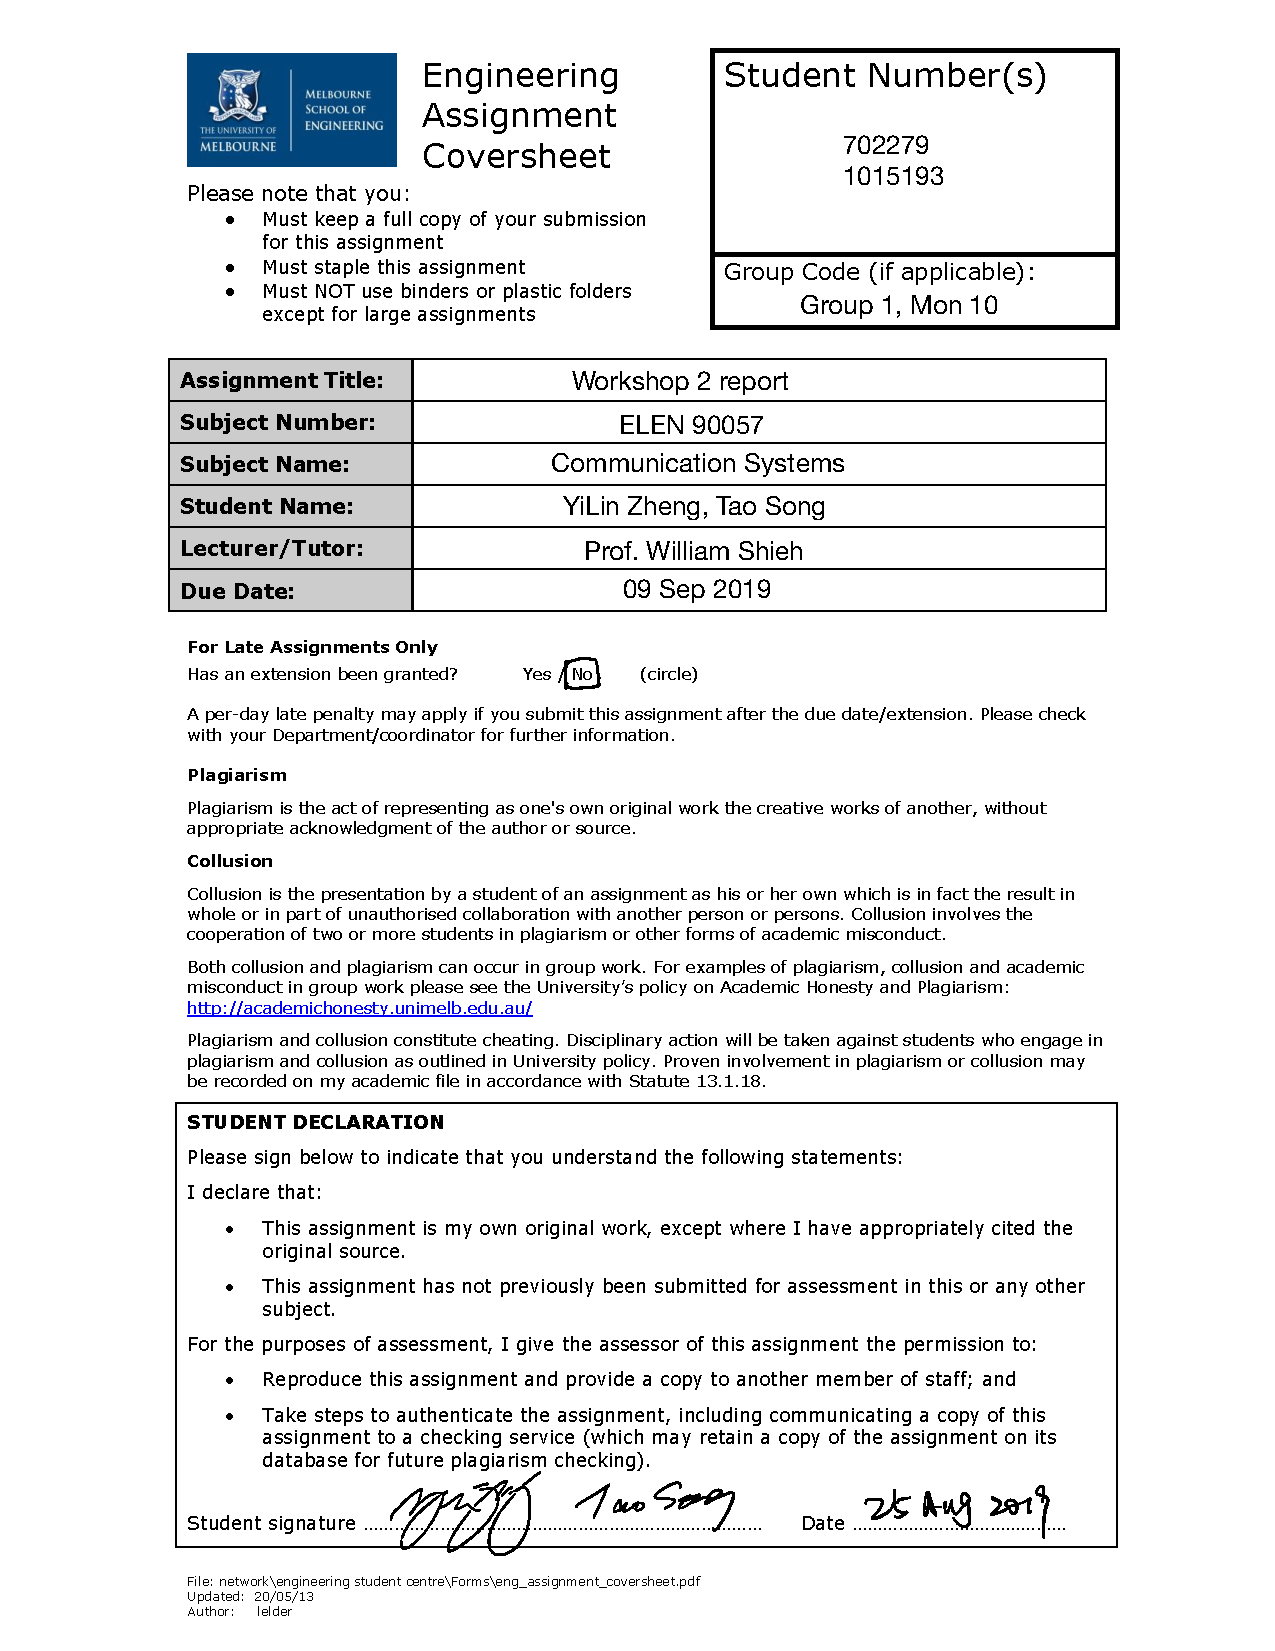
\includepdf{coverpagew2.pdf}
\newpage
\begin{center}
\textbf{\Large{Workshop 2}}\\
Group 1: Tao Song [1015193], YiLin Inez Zheng [702279], \\
Workshop: Monday 10:00am - 12:00pm (Shalanika, Bigi), Due: 09/09/19  
\end{center}


\section*{Question 1}
\begin{enumerate}[label=(\alph*)]
\item
The following table shows the information found on the relevant TIMS modules.
\begin{center}
 \begin{tabular}{|m{4cm}|m{3cm}|m{5.5cm}|m{2.5cm}|} 
 \hline
\textbf{TIMS modules} & \textbf{Voltage (V)} & \textbf{Frequency (Hz)} & \textbf{Gain}\\ 
 \hline
 Variable DC & Min -2.5, Max 2.5 & - & - \\
 \hline
 Master Signal & 4Vpp & 100kHz (carrier), 8.3333kHz (sample clock), 2.083kHz (audio) & - \\
 \hline
 Audio Oscillator & 4Vpp & Min 300Hz, Max 10kHz & - \\
 \hline
 Adder & Overloading will cause non-linear operation & - & Min 0, Max 2 \\
 \hline
 Multiplier & Output is scaled by 0.5 to avoid overloading & - & approx. 0.5 \\
 \hline
 Quadrature Adder & - & - & Min 0, Max 1.5 \\
 \hline
 Quadrature Multiplier & - & - & approx. 0.5 \\
 \hline
\end{tabular}
\end{center}

\end{enumerate}


\section*{Question 2}
\begin{enumerate}[label=(\alph*)]
\item From the given information, we have the expression for message signal $m(t)$ and carrier signal $v_c(t)$ as
    \begin{align*}
    m(t) &= \frac{1}{2} cos(2 \pi f_m t)+cos(2\pi 2 f_m t)\\
    v_c(t) &= A_c cos(2\pi f_c t)
    \end{align*}
thus, we have the DSB-SC signal $s(t)$ as
    \begin{align*}
    s(t) &=m(t)v_c(t) \\
    &= \biggr( \frac{1}{2} \cos(2 \pi f_m t)+\cos(2\pi 2 f_m t)\biggr )A_c \cos(2\pi f_c t)\\
    &=\frac{A_c}{2} \cos(2 \pi f_m t) \cos(2\pi f_c t)+ A_c \cos(2\pi 2 f_m t)\cos(2\pi f_c t)  \\
    &=\frac{A_c}{4}\biggr(\cos(2\pi f_c t - 2\pi f_m t) + \cos(2\pi f_c t + 2\pi f_m t) \biggr)\\ 
    &\hspace{1cm} + \frac{A_c}{2}\biggr( \cos(2\pi f_c t - 2\pi 2f_m t) + \cos(2\pi f_c t + 2\pi 2f_m t) \biggr)\\
    &= \frac{A_c}{4}\biggr(\cos(2\pi (f_c -f_m)t)+ \cos(2\pi (f_c +f_m)t) \biggr)\\
    &\hspace{1cm} + \frac{A_c}{2}\biggr( \cos(2\pi (f_c -2f_m)t)+ \cos(2\pi (f_c +2f_m)t) \biggr)\\
    &= \frac{A_c}{8} (e^{j2\pi (f_c-f_m) t}+e^{-j2\pi (f_c-f_m) t}+e^{j2\pi (f_c+f_m) t}+e^{-j2\pi (f_c+f_m) t})\\
    &\hspace{1cm} +\frac{A_c}{4}(e^{j2\pi (f_c - 2f_m) t}+e^{-j2\pi (f_c - 2f_m) t}+e^{j2\pi (f_c + 2f_m) t}+e^{-j2\pi (f_c+2f_m) t})
    \end{align*}
From here we observe,
\begin{itemize}
    \item % upper side band
    Upper side band: $\frac{A_c}{8} (e^{j2\pi (f_c+f_m)t} +  e^{-j2\pi (f_c+f_m)t}) + \frac{A_c}{4}(e^{j2\pi (f_c+2f_m)t} + e^{-j2\pi (f_c+2f_m)t})$
    \item % lower side band
    Lower side band: $\frac{A_c}{8} (e^{j2\pi(f_c-f_m)t} +  e^{-j2\pi (f_c-f_m)t}) + \frac{A_c}{4}(e^{j2\pi (f_c-2f_m)t} + e^{-j2\pi (f_c-2f_m)t})$
\end{itemize}
Taking Fourier transform of $s(t)$, we will have $S(f)$,
     \begin{align*}
    S(f)= \frac{A_c}{8} (\delta (f-(f_c-f_m)) +\delta (f+(f_c-f_m)) +\delta (f-(f_c+f_m)) +\delta (f+(f_c+f_m))\\
    +\frac{A_c}{4} (\delta (f-(f_c-2f_m)) +\delta (f+(f_c-2f_m)) +\delta (f-(f_c+2f_m)) +\delta (f+(f_c+2f_m))
    \end{align*}
By observing $S(f)$, there are 8 spikes throughout the entire spectrum. They are: 
\begin{multicols}{2}
\begin{itemize}
    \item $f_1=f_c-f_m$
    \item $f_2=-(f_c-f_m)$
    \item $f_3=f_c+f_m$
    \item $f_4=-(f_c+f_m)$
    \item $f_5=f_c-2f_m$
    \item $f_6=-(f_c-2f_m)$
    \item $f_7=f_c+2f_m$
    \item $f_8=-(f_c+2f_m)$
\end{itemize}
\end{multicols}
However, only four of them are located in passband (positive axis), the rest of them located in the LHS and are not meaningful ($f_2$, $f_4$, $f_6$, and $f_8$). Using the values of $f_c = 100$kHz and $f_m = 2$kHz, we expect peaks to be at 96kHz, 98kHz, 102kHz and 104kHz with magnitude of $\frac{A_c}{4}$,$\frac{A_c}{8}$,$\frac{A_c}{8}$ and $\frac{A_c}{4}$ respectively. 96kHz and 98kHz are the LSBs and 102kHz and 104kHz are the USBs.

\item % b & c
Figure \ref{fig:q2} shows the signal generated for both parts b) and c). The top half of the picture shows the DSBSC signal and the bottom half is the FFT output centered at 100kHz.
\begin{figure}[H]
    \centering
    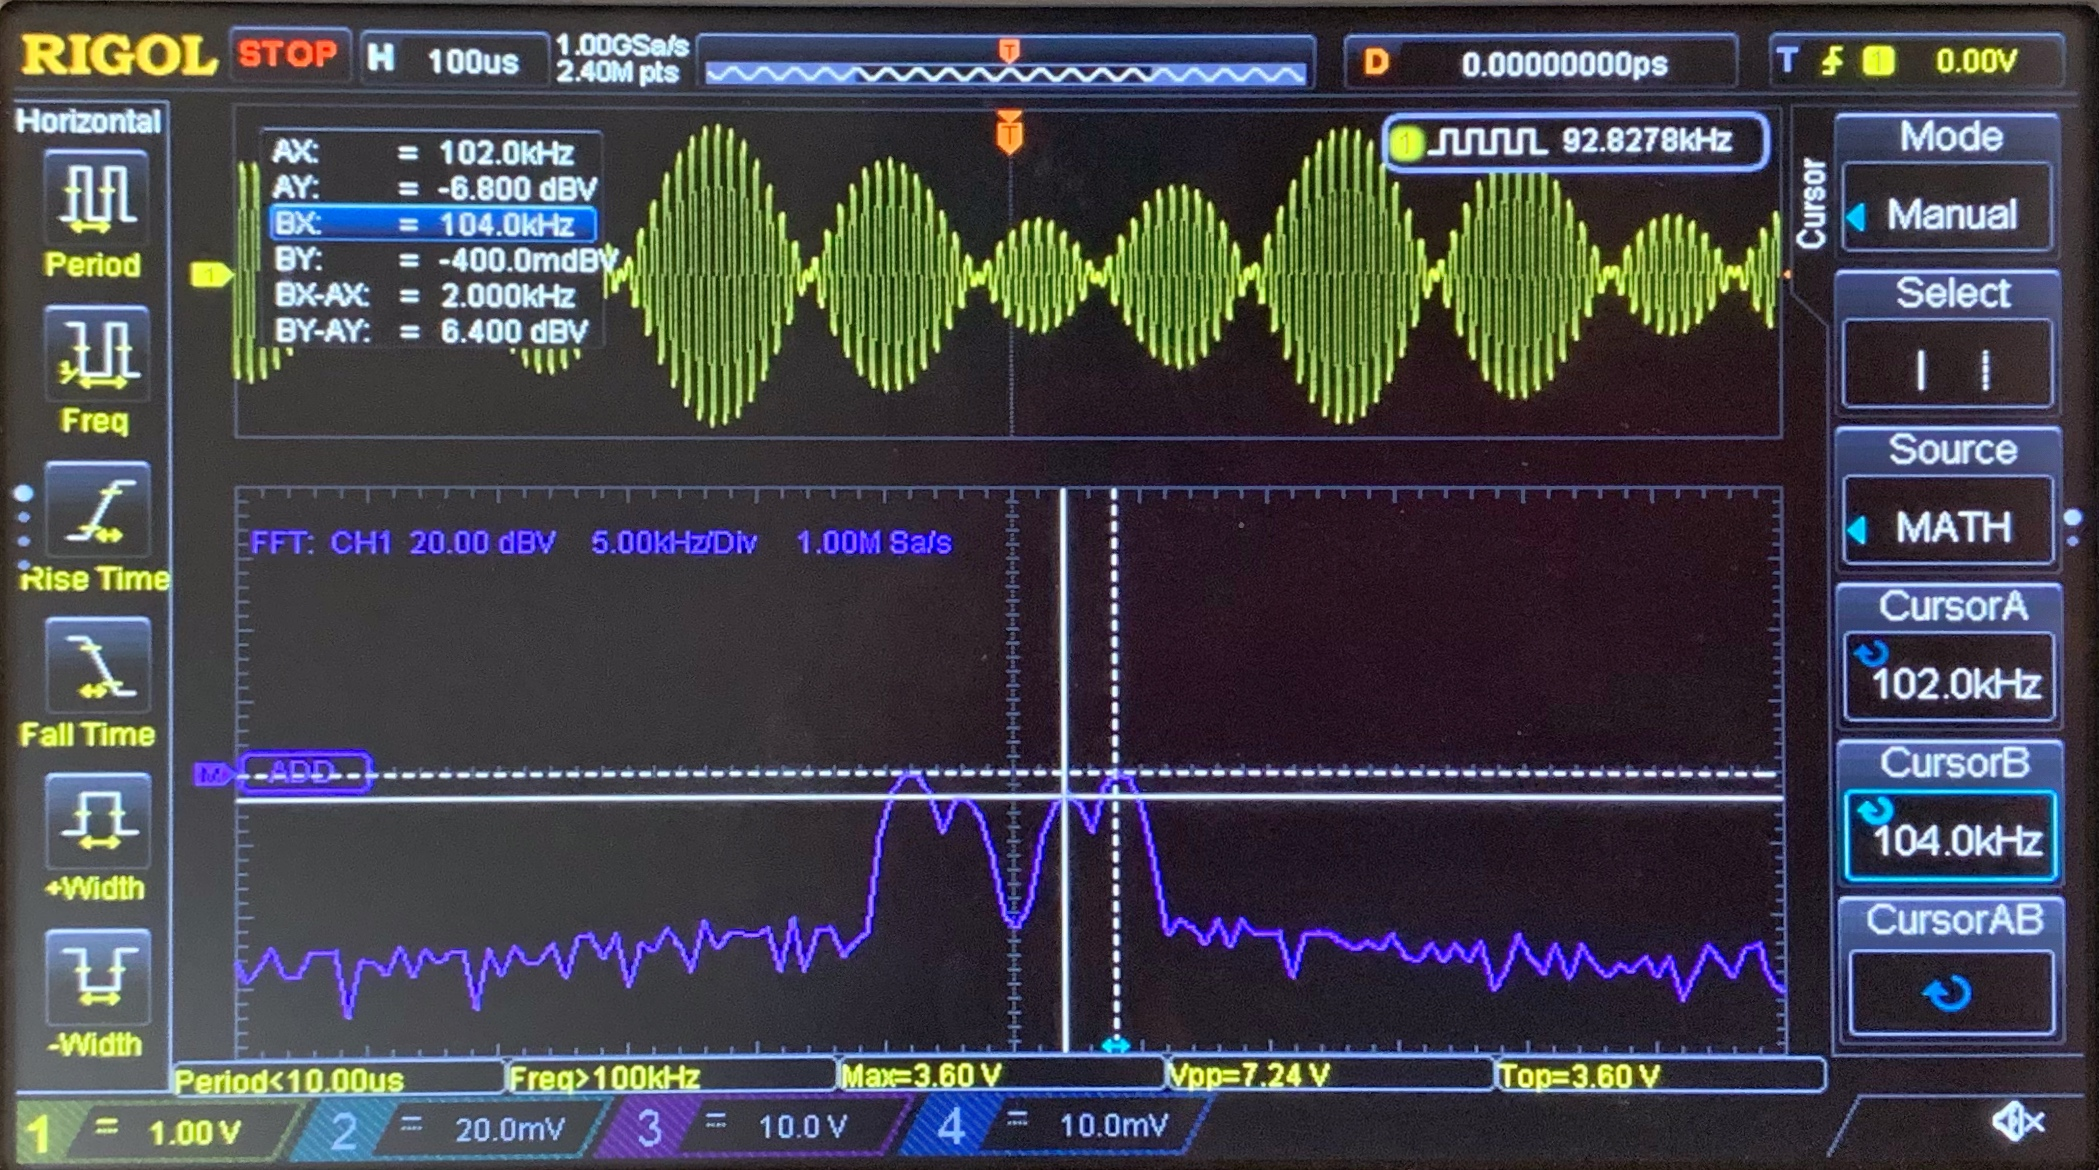
\includegraphics[scale = 0.205]{Q2b.jpg}
    \caption{\label{fig:q2}DSB-SC signal $s(t)$ in time domain and frequency domain}
\end{figure}

\newpage
\item %c explanation
It can be seen that the baseband signal has been successfully modulated into pass band (as shown in Figure \ref{fig:q2}). We had 4 spikes across the passband (located in 96kHz, 98kHz, 102kHz and 104kHz) which are expected from our calculations. The discrepancy here would be that the outcomes of the FFT only shows the real frequencies. In our calculations there were also negative frequency components of the DSBSC signal $S(f)$. In terms of magnitudes, the spikes on 98kHz and 102kHz were calculated to have half the magnitude of 96kHz and 104kHz peaks ($\frac{A_c}{8}$ compared to $\frac{A_c}{4}$). While the exact measurements from the experimental data did not show the difference as starkly (in dB 50\% $\approx$ 0.7). but it does indicate that the middle two spikes have a smaller magnitude. This might be due to the frequency components not being separate enough; they contribute to the magnitude of each other. We can't estimate this in our theoretical calculations as all the spikes are impulses in theory.

\item %d
We changed the frequency of the 4kHz (2$f_m$) signal in $m(t)$ to 10kHz to see the effects of the side lobes in the frequency spectrum. In Figure 2, we can see that the side lobes moved from 104kHz to 110kHz (measured but unfortunately the value is not displayed in figure) and in Figure 3, we can see that the taller side peaks previously had moved closer towards the centre frequency $f_c$ of 100kHz. The measurement of 100.8kHz shown isn't entirely accurate but is closer to 100.5kHz - what we were expecting (100kHz + 500Hz). Therefore, we get the observations of what we would expect when we change the frequency of message signal. With the specified frequency range of Audio Oscillator as shown in Question 1 (300Hz to 10kHz), we would only expect our passband to occupy the a frequency range of (80kHz - $f_c - 2f_m$,120kHz - $f_c + 2f_m$). By searching on the internet, AM radio signal will typically have a frequency of 540kHz and above. This indicates that our DSBSC signal will not interfere with AM radio signals and they are not even close.
\begin{figure}[H]
    \centering
    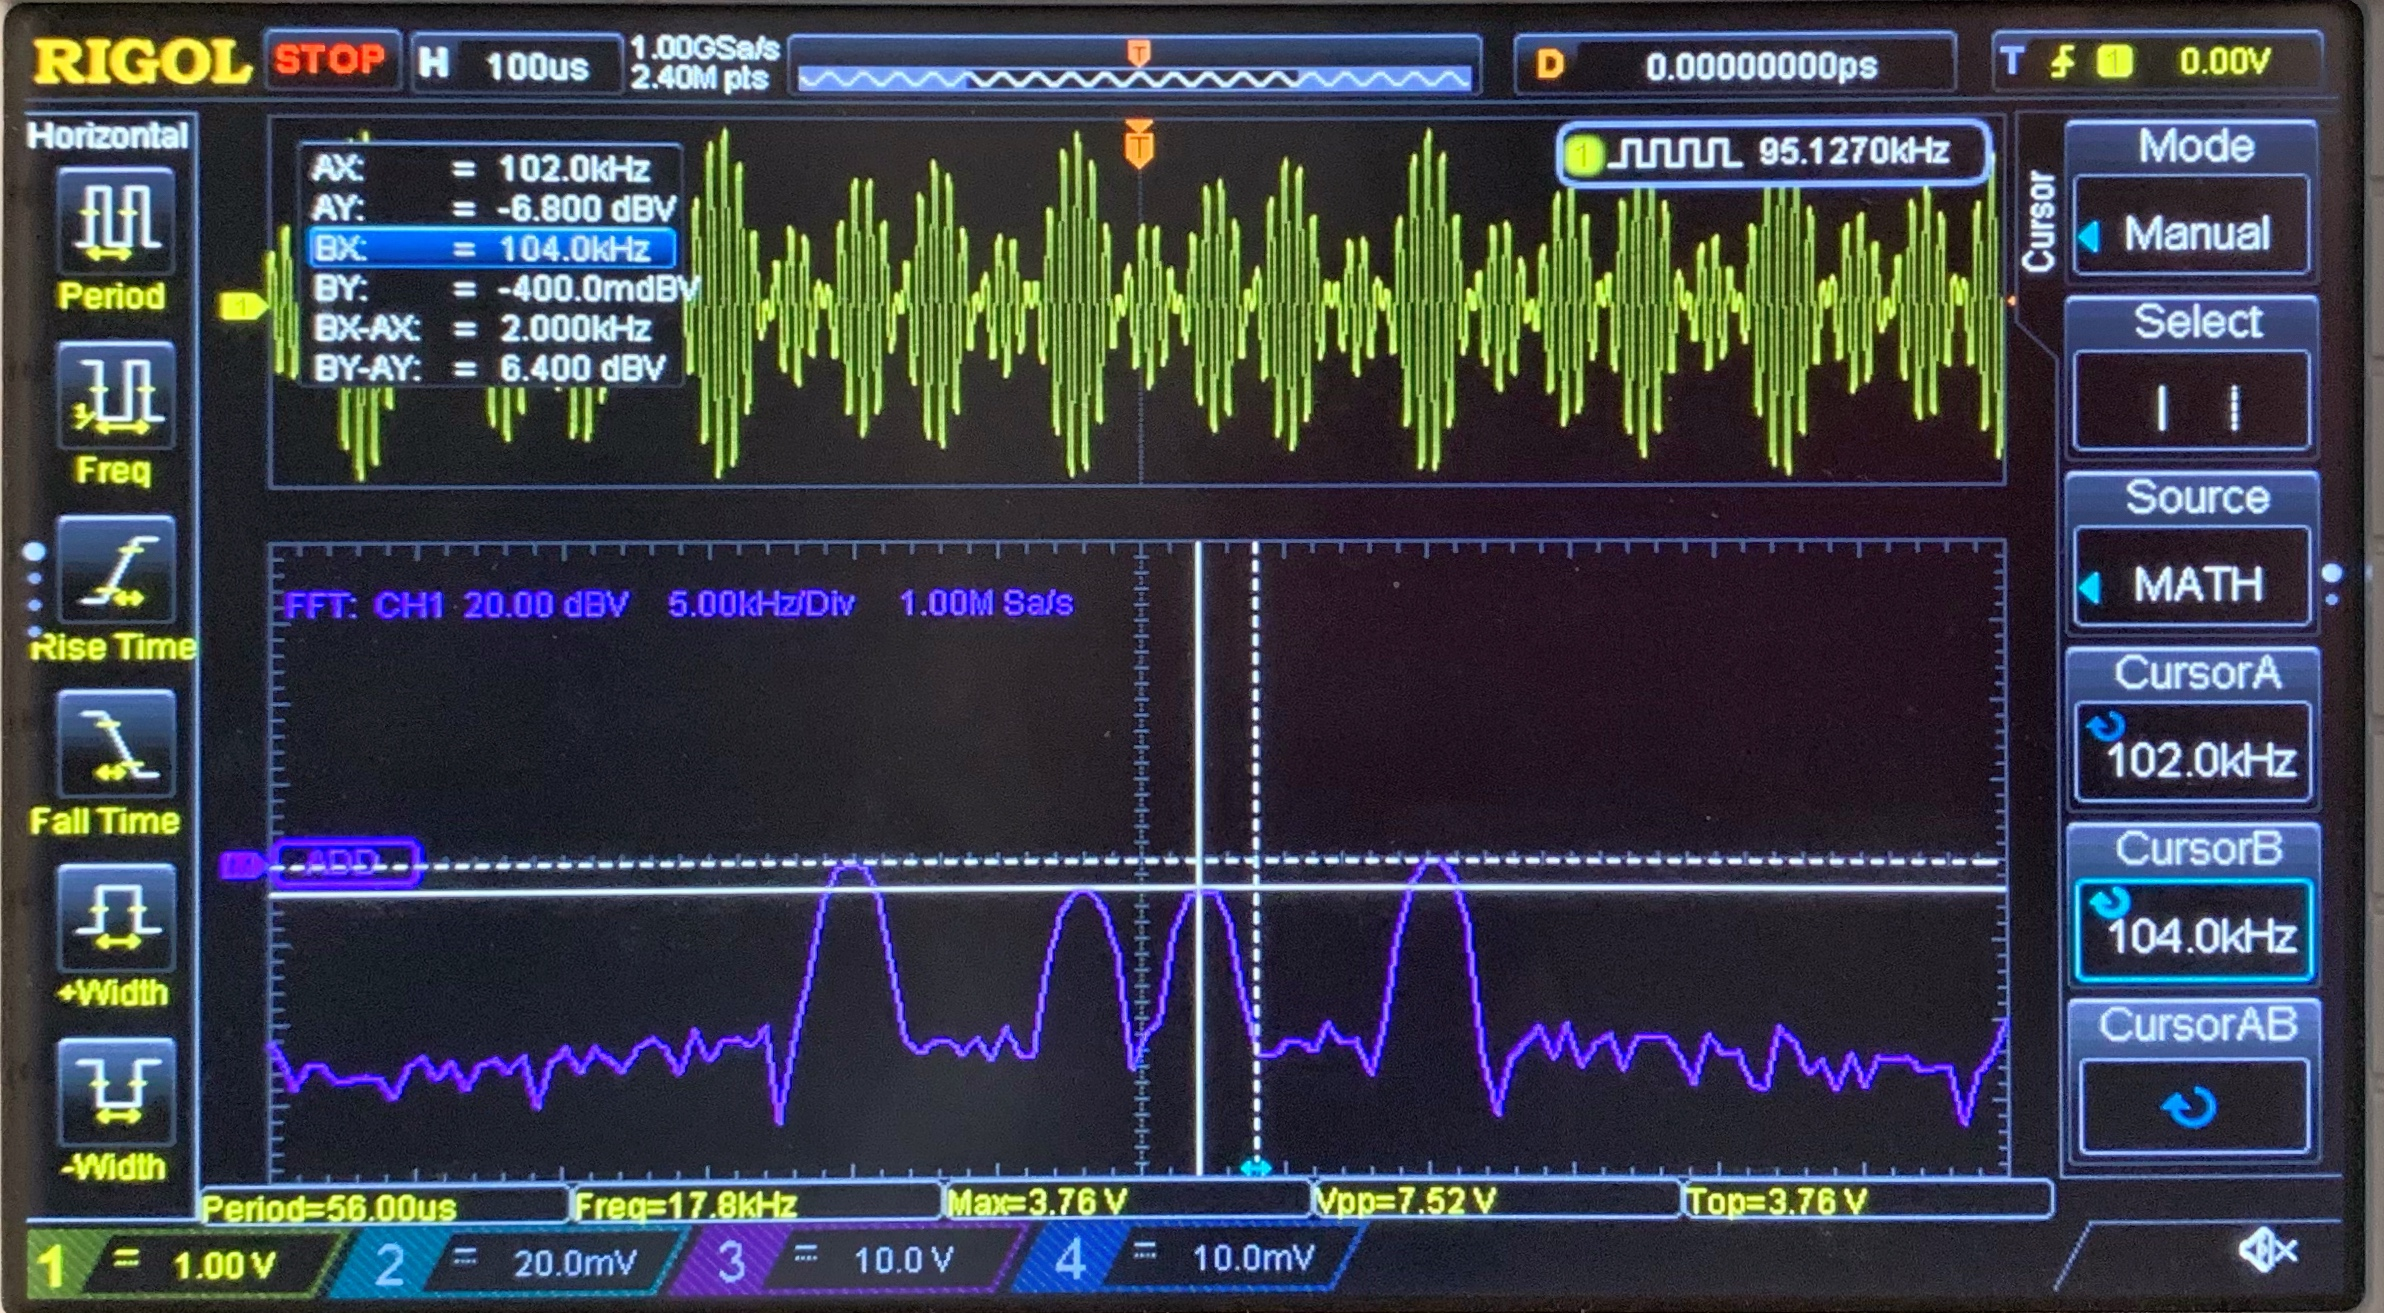
\includegraphics[scale = 0.18]{Q2d10kHz.jpg}
    \caption{\label{fig:q2d10k}DSB-SC signal $s(t)$ in time domain and frequency domain with the $2f_m$ signal at 10kHz}
\end{figure}
\begin{figure}[H]
    \centering
    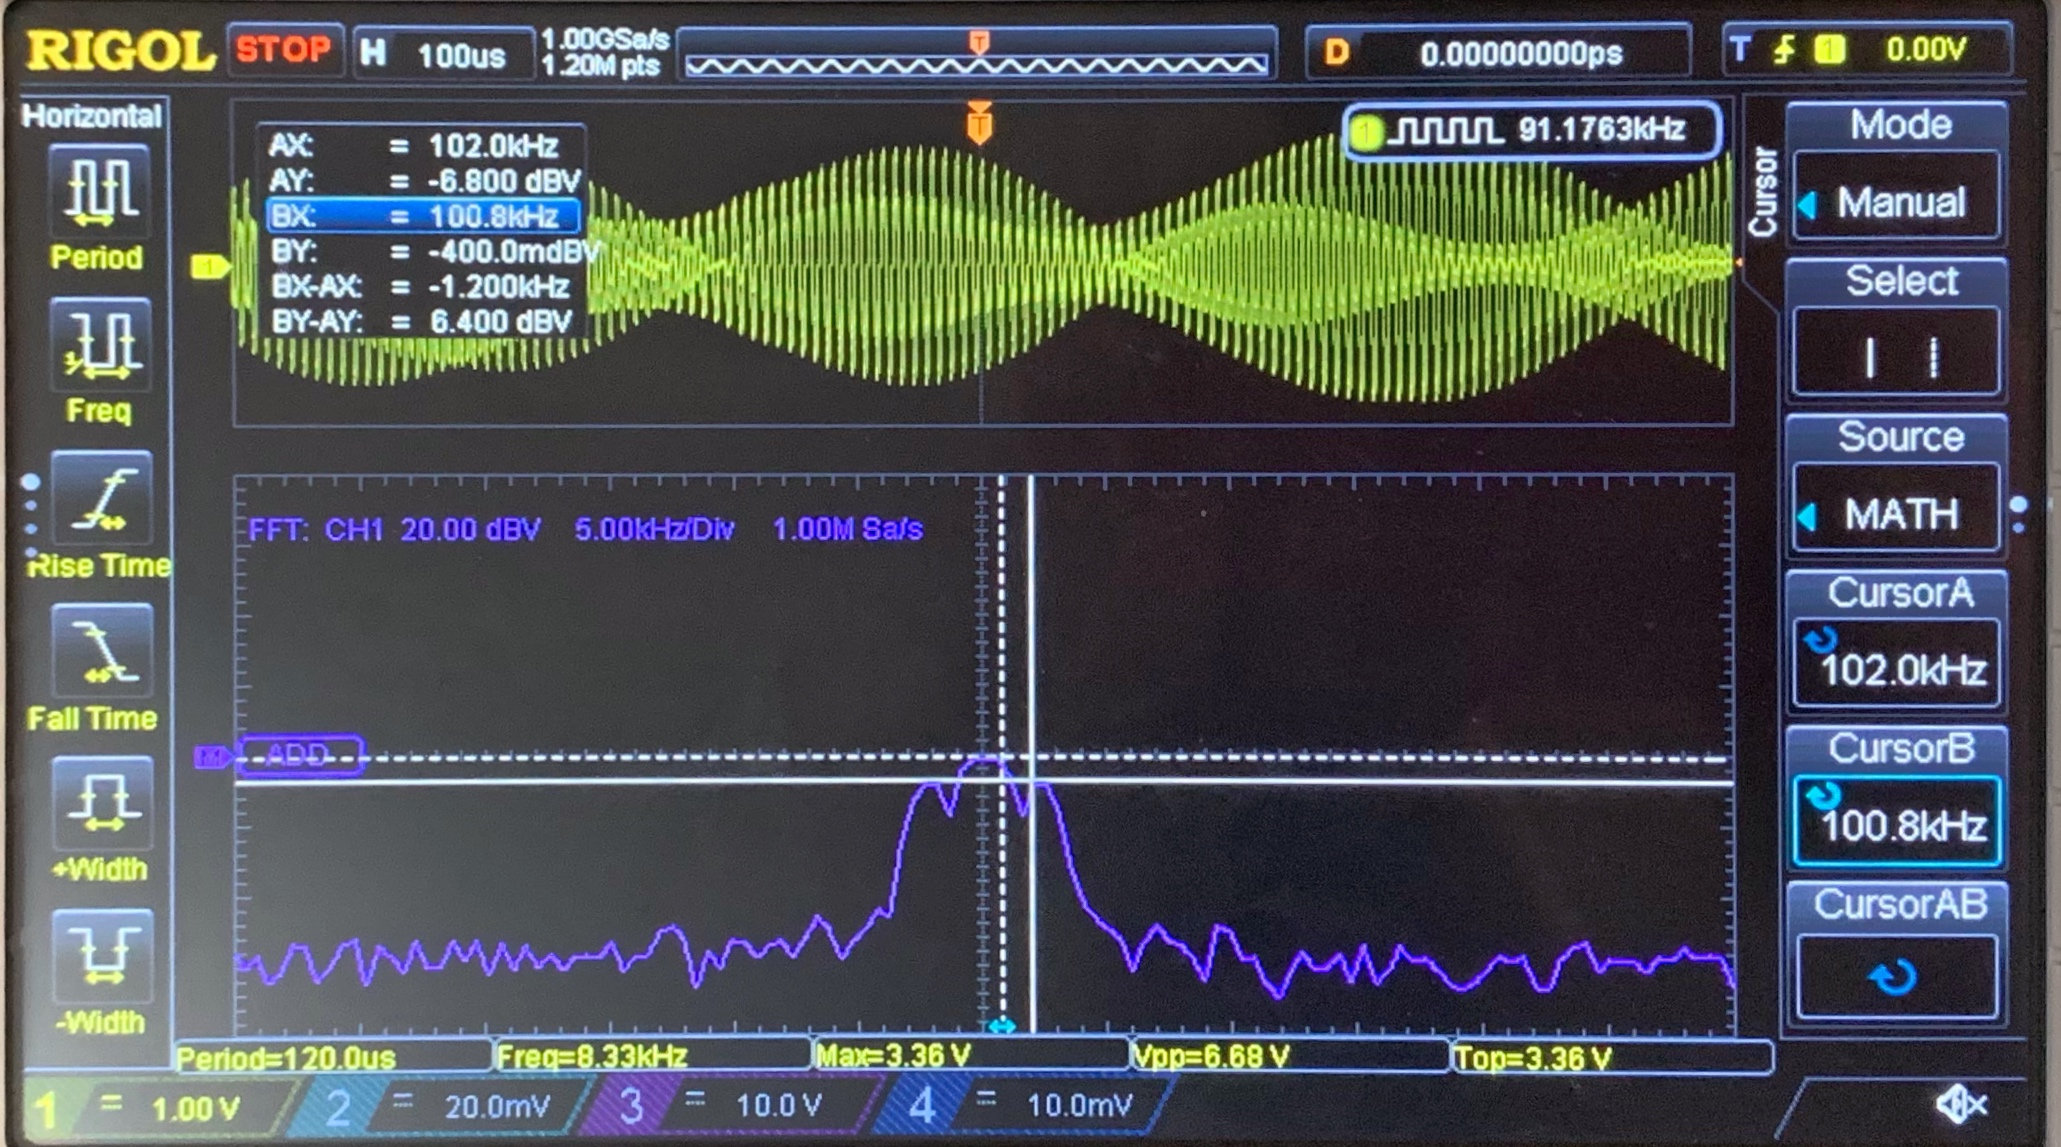
\includegraphics[scale = 0.21]{Q2d500Hz.jpg}
    \caption{\label{fig:q2d500}DSB-SC signal $s(t)$ in time domain and frequency domain with the $2f_m$ signal at 500Hz}
\end{figure}
\end{enumerate}

\section*{Question 3}
\begin{enumerate}[label=(\alph*)]
\item The received DSB-SC signal $s(t)$ is given from previous question as
     \begin{align*}
    s(t)=\frac{A_c}{4}\biggr(\cos(2\pi (f_c -f_m)t)+ \cos(2\pi (f_c +f_m)t) \biggr) + \frac{A_c}{2}\biggr( \cos(2\pi (f_c -2f_m)t)+ \cos(2\pi (f_c +2f_m)t) \biggr)
    \end{align*}
Using the stolen carrier $\tilde{v_c}(t)=A_c \cos(2\pi f_c t + \phi)$, the mixed signal will be
    \begin{align*}
    s(t)\tilde{v_c}(t)&=\frac{A_c^2}{4} \biggr(\cos(2\pi (f_c-f_m)t) \cos(2\pi f_c t + \phi) + \cos(2\pi (f_c+f_m)t) \cos(2\pi f_c t + \phi)) \biggr)\\
    &\hspace{1cm} + \frac{A_c^2}{2} \biggr(\cos(2\pi (f_c-2f_m)t) \cos(2\pi f_c t + \phi) + \cos(2\pi (f_c+2f_m)t) \cos(2\pi f_c t + \phi)) \biggr)\\
    &= \frac{A_c^2}{8} \biggr(\cos(2\pi (2f_c-f_m)t + \phi) + \cos(2\pi f_m t + \phi) + \cos(2\pi (2f_c+f_m)t + \phi) + \cos(2\pi f_m t - \phi)\biggr)\\
    &\hspace{1cm} + \frac{A_c^2}{4} \biggr(\cos(2\pi (2f_c-2f_m)t + \phi) + \cos(2\pi2f_m t + \phi)\\ 
    &\hspace{2cm} + \cos(2\pi (2f_c+2f_m)t + \phi) + \cos(2\pi 2f_m t - \phi) \biggr)
    \end{align*}
Since $\phi$ is considered small, we make a approximation of $\phi=0$ for easy calculations
    \begin{align*}
    s(t)\tilde{v_c}(t)&=\frac{A_c^2}{8} \biggr(\cos(2\pi (2f_c-f_m)t) + \cos(2\pi f_m t) + \cos(2\pi (2f_c+f_m)t) + \cos(2\pi f_m t)\biggr)\\
    &\hspace{1cm} + \frac{A_c^2}{4} \biggr(\cos(2\pi (2f_c-2f_m)t) + \cos(2\pi 2f_m t)+ \cos(2\pi (2f_c+2f_m)t) + \cos(2\pi 2f_m t) \biggr)\\ 
    &= \frac{A_c^2}{16} \biggr( e^{j2\pi (2f_c - f_m) t} + e^{-j2\pi (2f_c-f_m) t} + 2e^{j2\pi f_m t} + 2e^{-j2\pi f_m t} + e^{j2\pi (2f_c+f_m)t} + e^{-j2\pi (2f_c+f_m)t} \biggr)\\
    &\hspace{1cm} +\frac{A_c^2}{8} \biggr( e^{j2\pi (2f_c - 2f_m) t} + e^{-j2\pi (2f_c-2f_m) t} + 2e^{j2\pi 2f_m t}\\ 
    &\hspace{2cm} + 2e^{-j2\pi 2f_m t} + e^{j2\pi (2f_c+2f_m)t} + e^{-j2\pi (2f_c+2f_m)t} \biggr) 
    \end{align*}
To find the frequency domain expression for the mixed signal, we take Fourier transform of $s_1 (t)\tilde{v_c}(t)$
\begin{align*}
    S(f)\tilde{V_c}(f)&= \frac{A_c^2}{16} \biggr(\delta(f-(2f_c-f_m)) + \delta(f+(2f_c-f_m))+2\delta(f-f_m)+2\delta(f+f_m)\biggr)\\
    &\hspace{1cm} +\frac{A_c^2}{8} \biggr( \delta(f-(2f_c-2f_m)) + \delta(f+(2f_c-2f_m))+2\delta(f-2f_m)+2\delta(f+2f_m) \biggr)
\end{align*}
By observing the frequency domain expression, we can see that there are 12 spikes across the entire spectrum. Again like previously in Q2, only 6 spikes should be in the RHS. Substituting in the values of $f_c$ and $f_m$, we should expect spikes at: 2kHz, 4kHz, 196kHz, 198kHz, 202kHz and 204kHz.\\ 
We forgot to take a picture of the full spectrum here but the experimental peaks were as expected. We have a picture of Figure \ref{fig:q3a} showing just the base band peaks at 2kHz and 4kHz which we demodulated in the next section using a LPF. All experimental data is checked off by our demonstrator.
\begin{figure}[H]
    \centering
    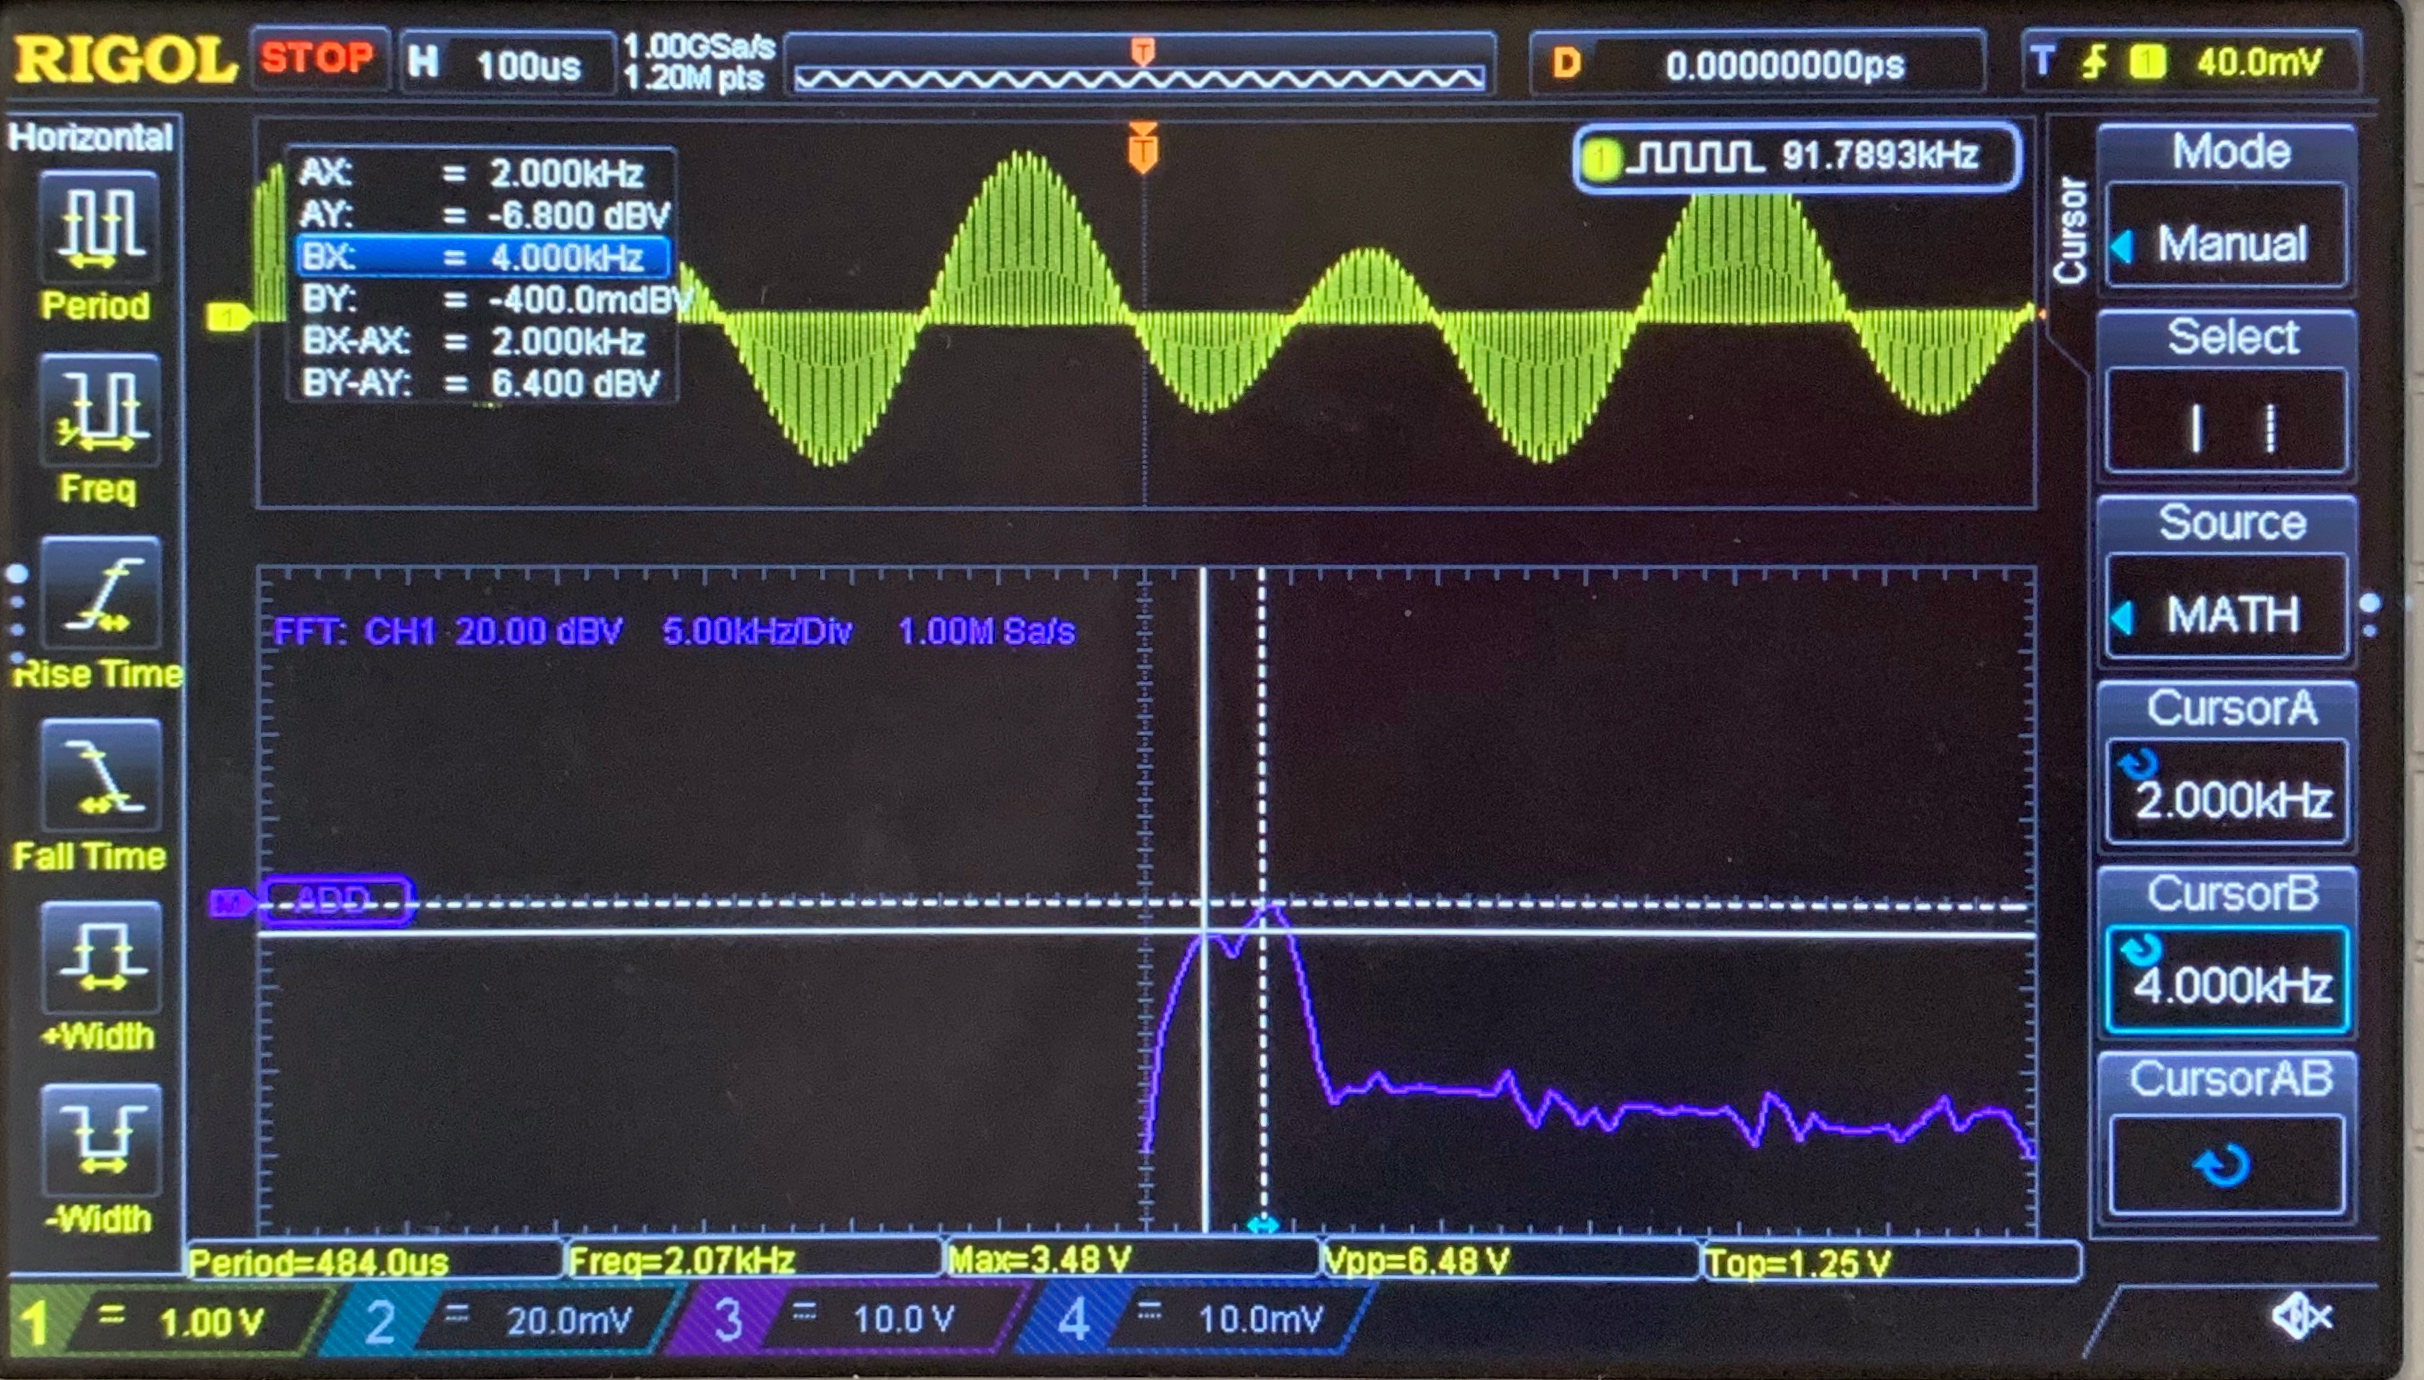
\includegraphics[scale = 0.16]{Q3a.jpg}
    \caption{\label{fig:q3a}DSB-SC demodulation after passing through low pass filter in time domain and frequency domain.}
\end{figure}

\item %b
From the above calculated expression for the spectrum, we would only interested in the frequency components that are located in the baseband ($-2f_m$ to $2f_m$). Therefore, the bandwidth $B$ should be greater than the baseband range will much smaller than the next un-interested frequency components ($f_c - 2f_m$). In summary bandwidth should maintain:
\begin{align*}
    2f_m<B<< f_c - 2f_m\\
    4\text{kHz}<B<<196\text{kHz}
\end{align*}

\item %c
Figure \ref{fig:q3c} shows our demodulation using a stolen carrier frequency after passing through a 60kHz LPF. The light blue (CH2) signal is $m(t)$, the original message and the yellow (CH1) signal is the recovered output signal. It can be seen in time domain, the demodulated signal are quite in phase with the original signal. In frequency domain, it showed two spikes located in 2kHz and 4kHz which are as same as the message signal. This indicates a very good demodulation of the received DSBSC signal. From theoretical calculations, the spike at 2kHz should have half magnitude of the spike at 4Hz. However, the spike at 2kHz is only slightly lower than the spike at 4Hz in our experimental results, which can be attributed into experimental instruments/setting errors. 
\begin{figure}[H]
    \centering
    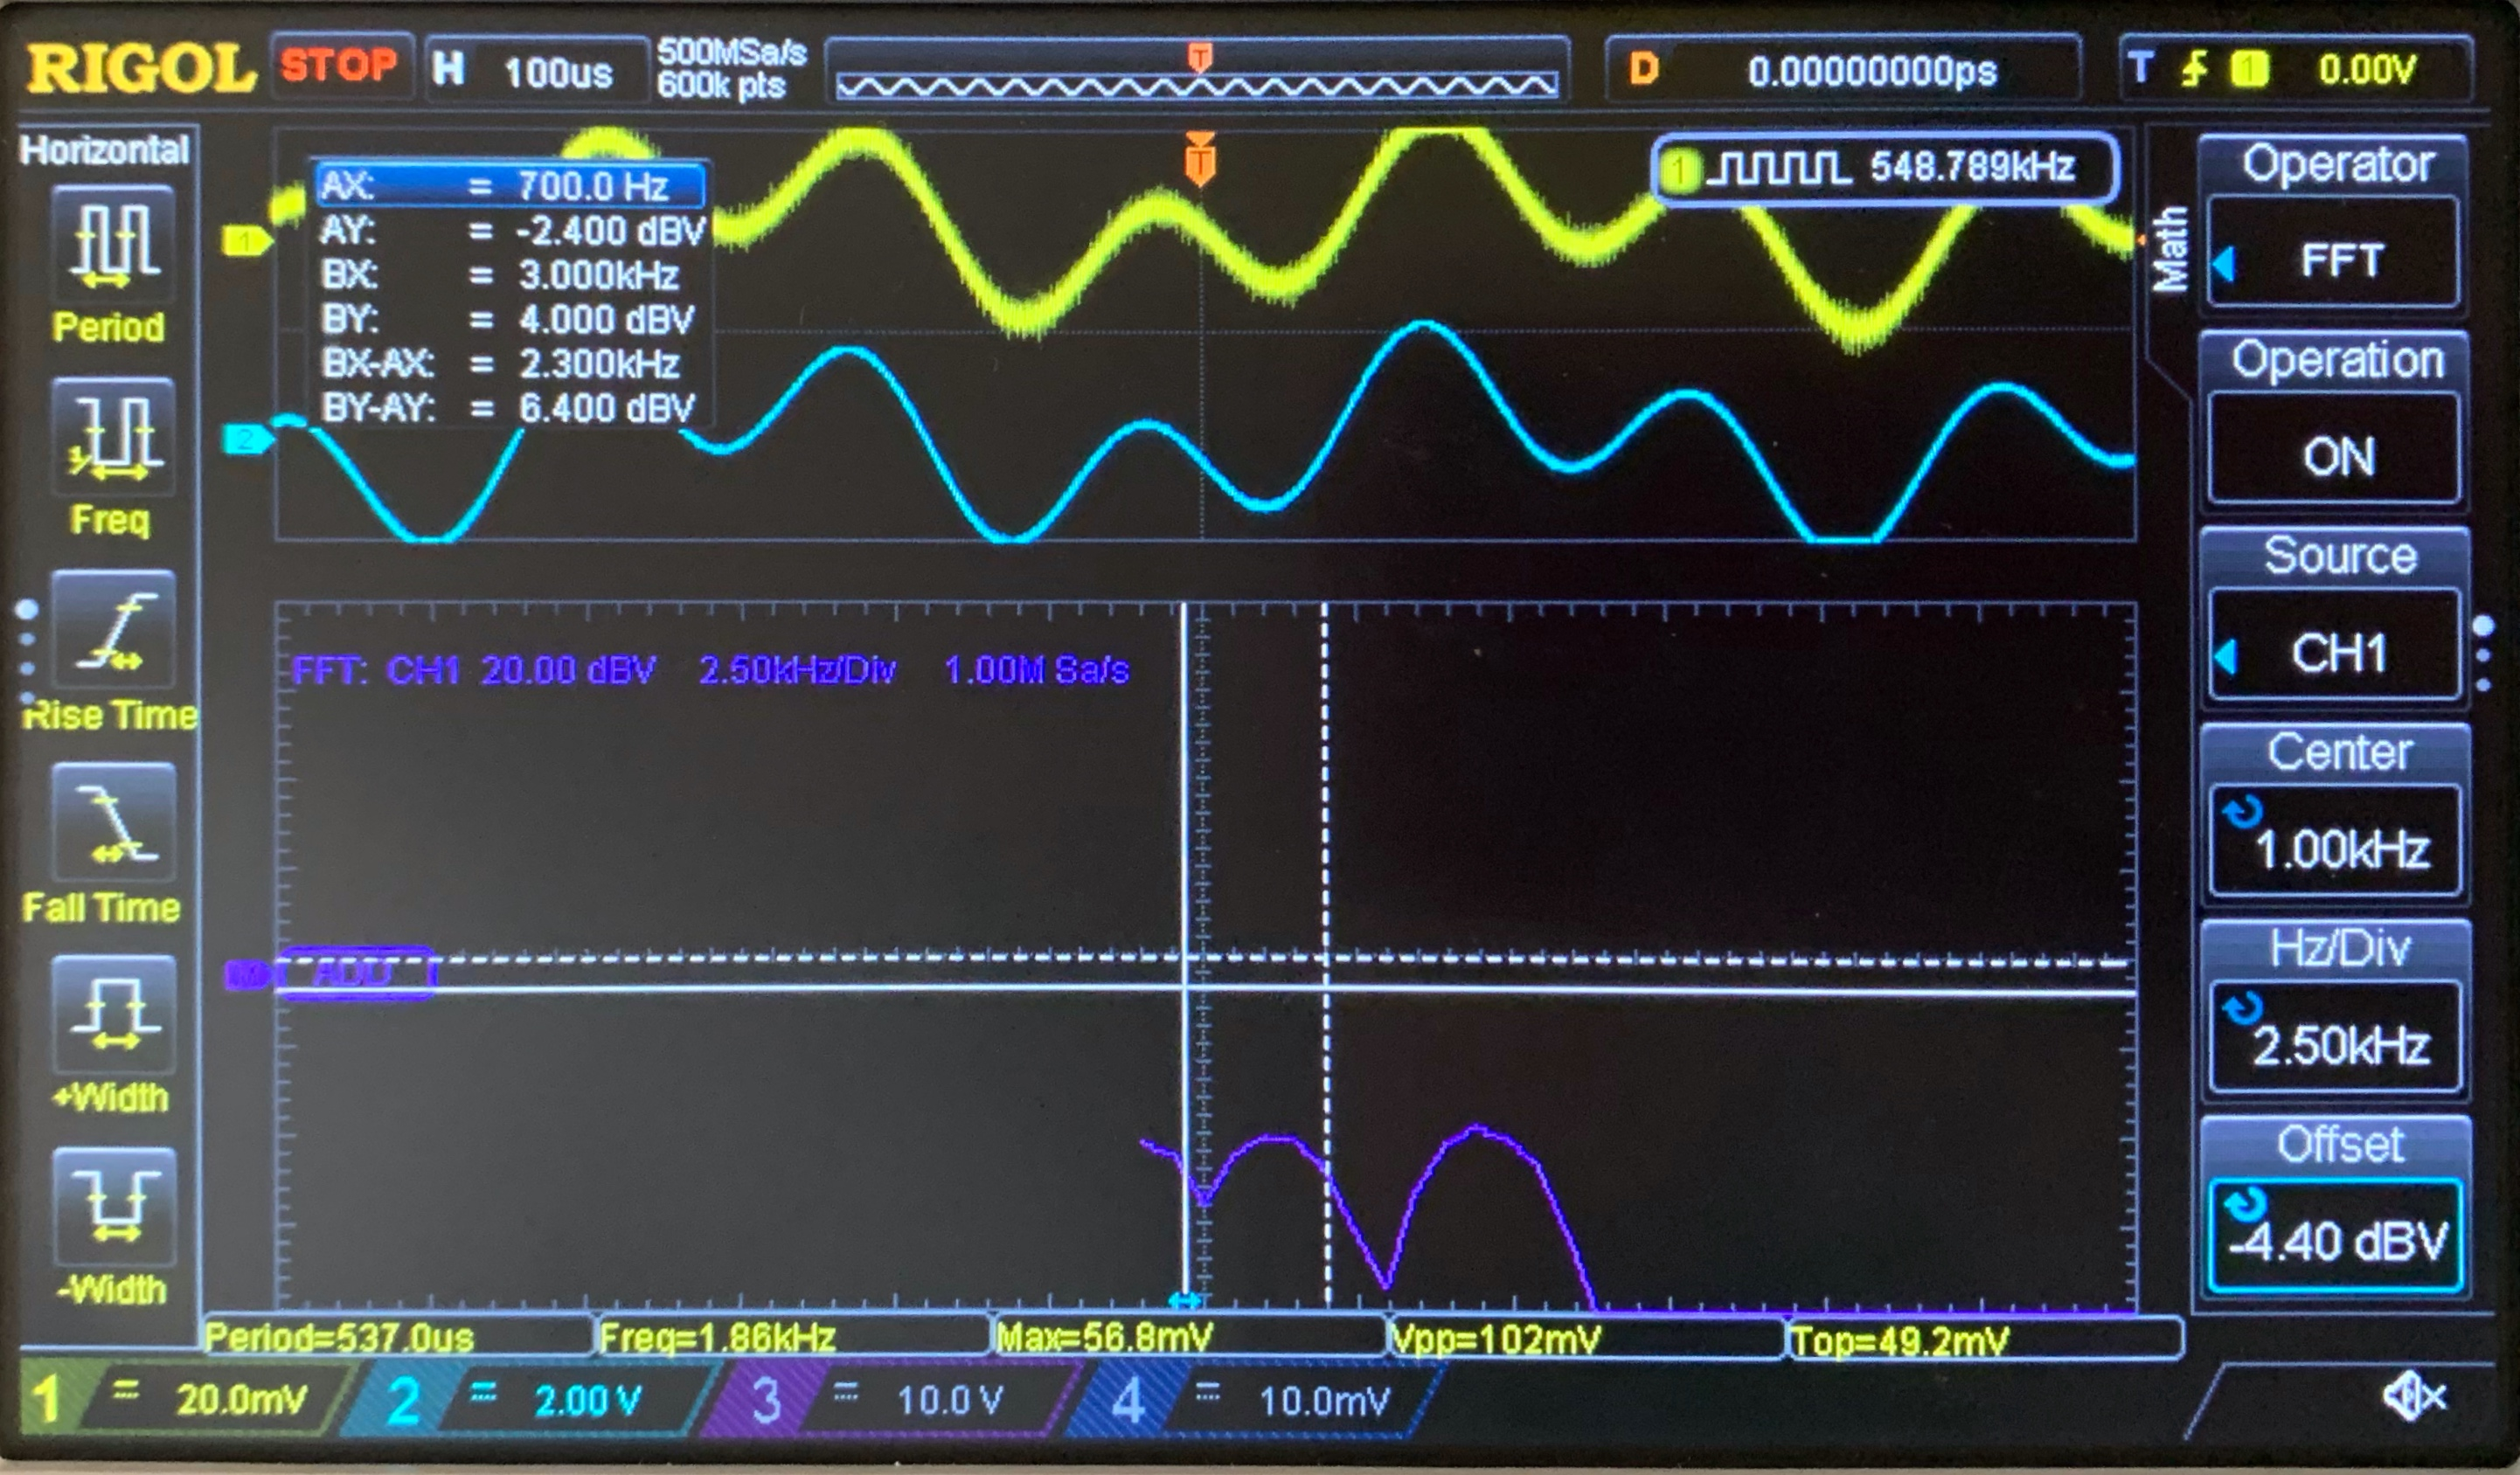
\includegraphics[scale = 0.135]{Q3c.jpg}
    \caption{\label{fig:q3c}Demodulated DSB-SC signal in time domain and frequency domain comparing with the original message signal $m(t)$}
\end{figure}

\item %d 
The Hilbert transform in the frequency domain is simply $-j\sgn(f)S(f)$. The time-domain expression for Hilbert transform of $s(t)$ is denoted as $\tilde{s} (t)$ below,
\begin{align*}
\tilde{s_1} (t)&=s(t)\ast \frac{1}{\pi t}\\
            &= \Biggr( \frac{A_c}{2} \cos(2\pi f_m t) \cos(2\pi f_c t)+ A_c \cos(2\pi 2 f_mt) \cos(2\pi f_c t) \Biggr) \ast \frac{1}{\pi t} \\
            & = \Biggr[ \frac{A_c}{4} (\cos(2\pi (f_c + f_m) t) + \cos(2\pi (f_c - f_m) t))+ \frac{A_c}{2} (\cos(2\pi (f_c + 2f_m) t) + \cos(2\pi (f_c - 2f_m) t)) \Biggr] \ast \frac{1}{\pi t}\\
            &= \frac{A_c}{4} (\sin(2\pi (f_c + f_m) t) + \sin(2\pi (f_c - f_m) t))+ \frac{A_c}{2} (\sin(2\pi (f_c + 2f_m) t) + \sin(2\pi (f_c - 2f_m) t))\\
            &= A_c \sin(2\pi f_ct)\biggr[\frac{1}{2}\cos(2\pi f_m t) + \cos(2\pi 2f_m t) \biggr]
\end{align*}
We omitted the $\sgn(t)$ from above due to our signal being causal and real, therefore we only observed it in the frequency domain for $f>0$, where $\sgn(f) = 1$. The Hilbert Transform after demodulation gives $m(t)$ at a scale of $A_c^2$,
\begin{align*}
    s(t)A_c \cos(2\pi f_ct) &+ \tilde{s}(t)A_c \sin(2\pi f_ct)\\ 
    &= m(t)A_c \cos(2\pi f_ct)A_c \cos(2\pi f_ct) + m(t)A_c \sin(2\pi f_ct)A_c \sin(2\pi f_ct)\\
    &= A_c^2 m(t)
\end{align*}

\item %e
The following figure shows our demodulation using the Hilbert Transform. The light blue (CH2) signal is $m(t)$, the original message and the yellow (CH1) signal is the recovered output. As seen from Figure \ref{fig:q3e}, the Hilbert transform gives an amplitude boost compared to the DSBSC demodulation $m(t)$. The original signal only recovered from DSBSC has an amplitude of $\frac{A_c^2}{2}$ whereas the Hilbert transform recovered signal has an amplitude of $A_c^2$.
\begin{figure}[H]
    \centering
    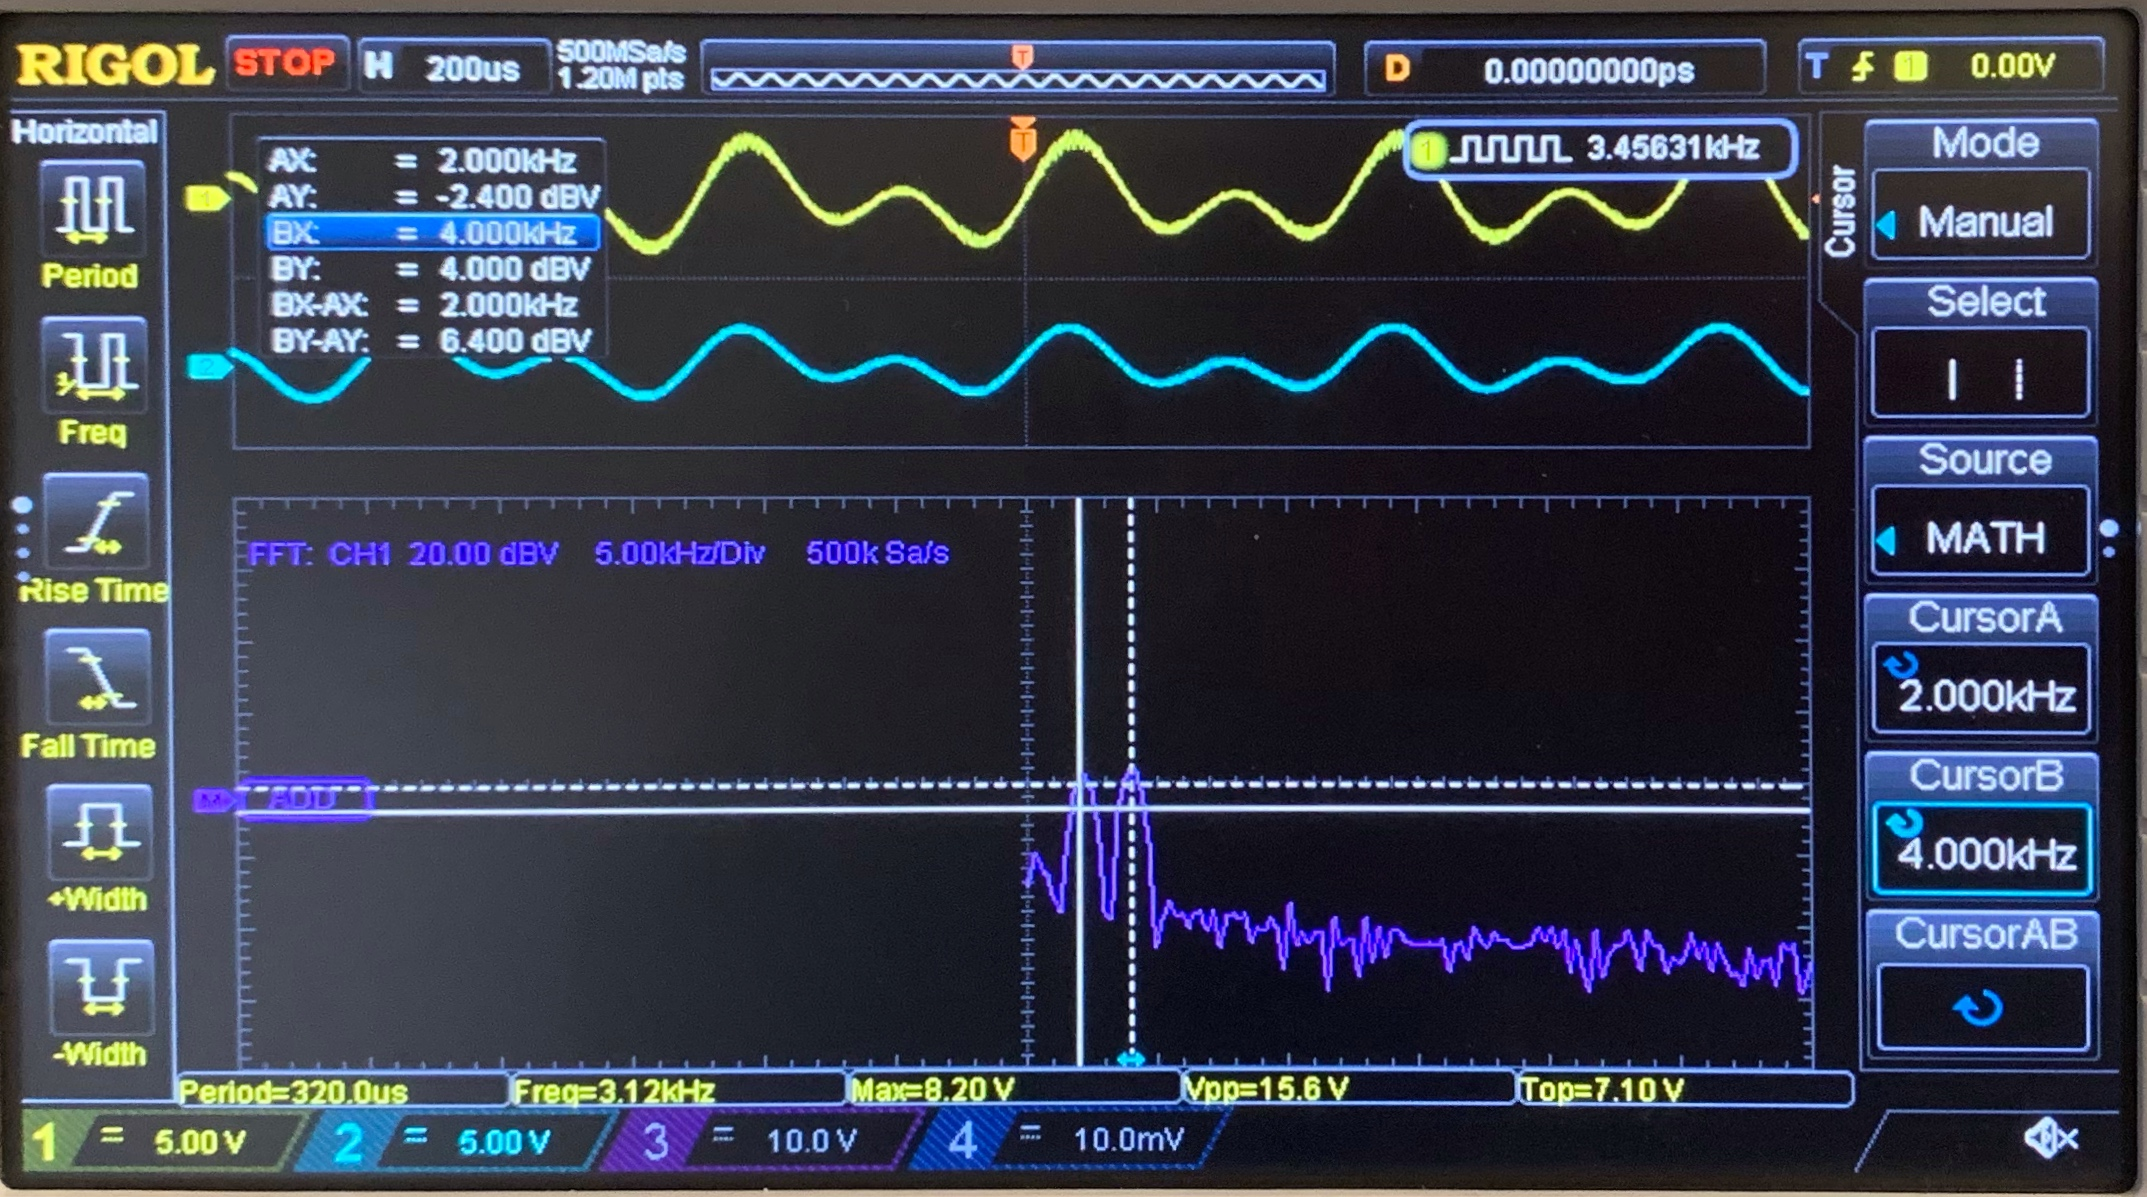
\includegraphics[scale = 0.20]{Q3e.jpg}
    \caption{\label{fig:q3e}Demodulated DSB-SC signal in time domain and frequency domain comparing with the original message signal $m(t)$}
\end{figure}
\end{enumerate}

%%%%%%% so far so good.

\section*{Question 4}
\begin{enumerate}[label=(\alph*)]
\item %a
To have DSB-SC changed to AM, we can look into their math expressions: 
\begin{align*}
\text{DSB-SC}&: s(t) = A_c m(t)\cos(2\pi f_c t) = A_c\biggr( \frac{1}{2} \cos(2 \pi f_m t)+\cos(2\pi 2 f_m t)\biggr ) \cos(2\pi f_c t)\\
\text{AM}&: s_{AM}(t) = A_c \biggr(1+\mu m(t) \biggr)\cos(2\pi f_c t) = A_c \cos(2\pi f_c t)+\mu s(t)
\end{align*}
this indicates us that AM can be achieved by giving a variable gain (which is $\mu$) to $s(t)$ and use system adder to add a carrier signal. There are three constrains for modulation index $\mu$:
\begin{align*}
 & 1+\mu m(t)_{min}>0\\
 & \mu<\frac{1}{|m(t)|}\\
 & \mu<1
\end{align*}
to solve these constrains, we need to firstly look into $m(t)$
\begin{align*}
 m(t)&=\frac{1}{2} \cos(2 \pi f_m t)+\cos(2\pi 2 f_m t) \\
 &= \frac{1}{2} \cos(2 \pi f_m t)+2\cos^2(2\pi f_m t)-1\\
 &=2(\cos(2\pi f_m t)+\frac{1}{8})^2-\frac{33}{32}
\end{align*}
this yields a minimum for $m(t)$ to be $-\frac{33}{32}$ when $\cos(2\pi f_m t)=-\frac{1}{8}$. Substitute this into the first constrain, we will have $\mu<\frac{32}{33}$, which also satisfy the rest two constrains. Note that we want to have the largest value of $\mu$ from the first two constrains whilst satisfying the last constrain. To have the largest value from the second constrain, we will need to have $\mu<\frac{1}{m(t)_{min}}$ which gives us $m<\frac{32}{33}$ as well. Thus we can say that the largest theoretical value of $\mu$ is $\frac{32}{33}$.

\item %b
The AM modulated signal $s_2 (t)$ with modulation index larger and smaller than the maximum value are shown in Figure \ref{fig:q4blarge} and Figure \ref{fig:q4bsmall} respectively. With $\mu$ in a desired range (smaller than its maximum value), $s_2 (t)$ will have 5 frequency components: one in carrier frequency ($f_c=100kHz$) and two pairs of frequency components symmetric with respect to the carrier frequency ($f_c=100kHz$).\\
Recall what we had for the amplitude modulation:
\begin{align*}
    s_{AM}(t)& = A_c \cos(2\pi f_c t)+\mu s(t) \\
    &= \frac{A_c}{2} (e^{j2\pi f_c t}+e^{-j2\pi f_c t})+\mu s(t)
\end{align*}
Take Fourier transform we will have
\begin{align*}
    S_{AM}(f) = \frac{A_c}{2} \delta(f-f_c)+\frac{A_c}{2}\delta(f+f_c) +\mu\frac{A_c}{8} \delta (f-(f_c-f_m)) +\mu\frac{A_c}{8}\delta (f+(f_c-f_m)) \\ + \mu\frac{A_c}{8}\delta (f-(f_c+f_m)) + \mu\frac{A_c}{8}\delta (f+(f_c+f_m))
    +\mu\frac{A_c}{4} (\delta (f-(f_c-2f_m)) \\ +\mu\frac{A_c}{4}\delta (f+(f_c-2f_m)) +\mu\frac{A_c}{4}\delta (f-(f_c+2f_m)) +\mu\frac{A_c}{4}\delta (f+(f_c+2f_m)))
\end{align*}

Leaving those frequency components that we are interested in (positive $f$), we have
\begin{align*}
    S_{AM}(f) = \frac{A_c}{2} \delta(f-f_c)+ \frac{\mu A_c}{8}\delta (f-(f_c-f_m)) + \frac{\mu A_c}{8} \delta (f-(f_c+f_m)) \\ +\frac{\mu A_c}{4}\delta (f-(f_c-2f_m)) +\frac{\mu A_c}{4} \delta (f-(f_c+2f_m) 
\end{align*}
this indicates that we should have five spikes which are located in:
\begin{multicols}{3}
\begin{itemize}
    \item $f_1=f_c=100$kHz
    \item $f_2=f_c-f_m=98$kHz
    \item $f_3=f_c+f_m=102$kHz
    \item $f_4=f_c+2f_m=104$kHz
    \item $f_5=f_c-2f_m=96$kHz
\end{itemize}
\end{multicols}
We had exactly 5 spikes from the experimental results as shown in Figure \ref{fig:q4blarge}, from which we can also find that the middle three spikes are quite well matching the calculations. The two spikes on each side are at $96kHz$ and $104kHz$, whilst the further two bands resemble $93kHz$ and $107kHz$ shown in the figure. This "discrepancy" with the expectation is due to our demonstrator shifting around our 4kHz message signal to test the separation and match between the graphs. The point at which we captured this image what when the tuning stopped the original 4kHz signal at 7kHz and therefore the graph still exhibits our experimental data reflecting theory. In terms of magnitude, the spike in very middle has the largest magnitude as $\frac{\mu A_c}{2}$. The two spikes located in 102kHz and 98kHz have the smallest magnitude which is half of the two spikes located in 96kHz and 104kHz. The tendency can be observed from our experimental results while the precise magnitudes are not as accurate as calculations. 
\begin{figure}[H]
    \centering
    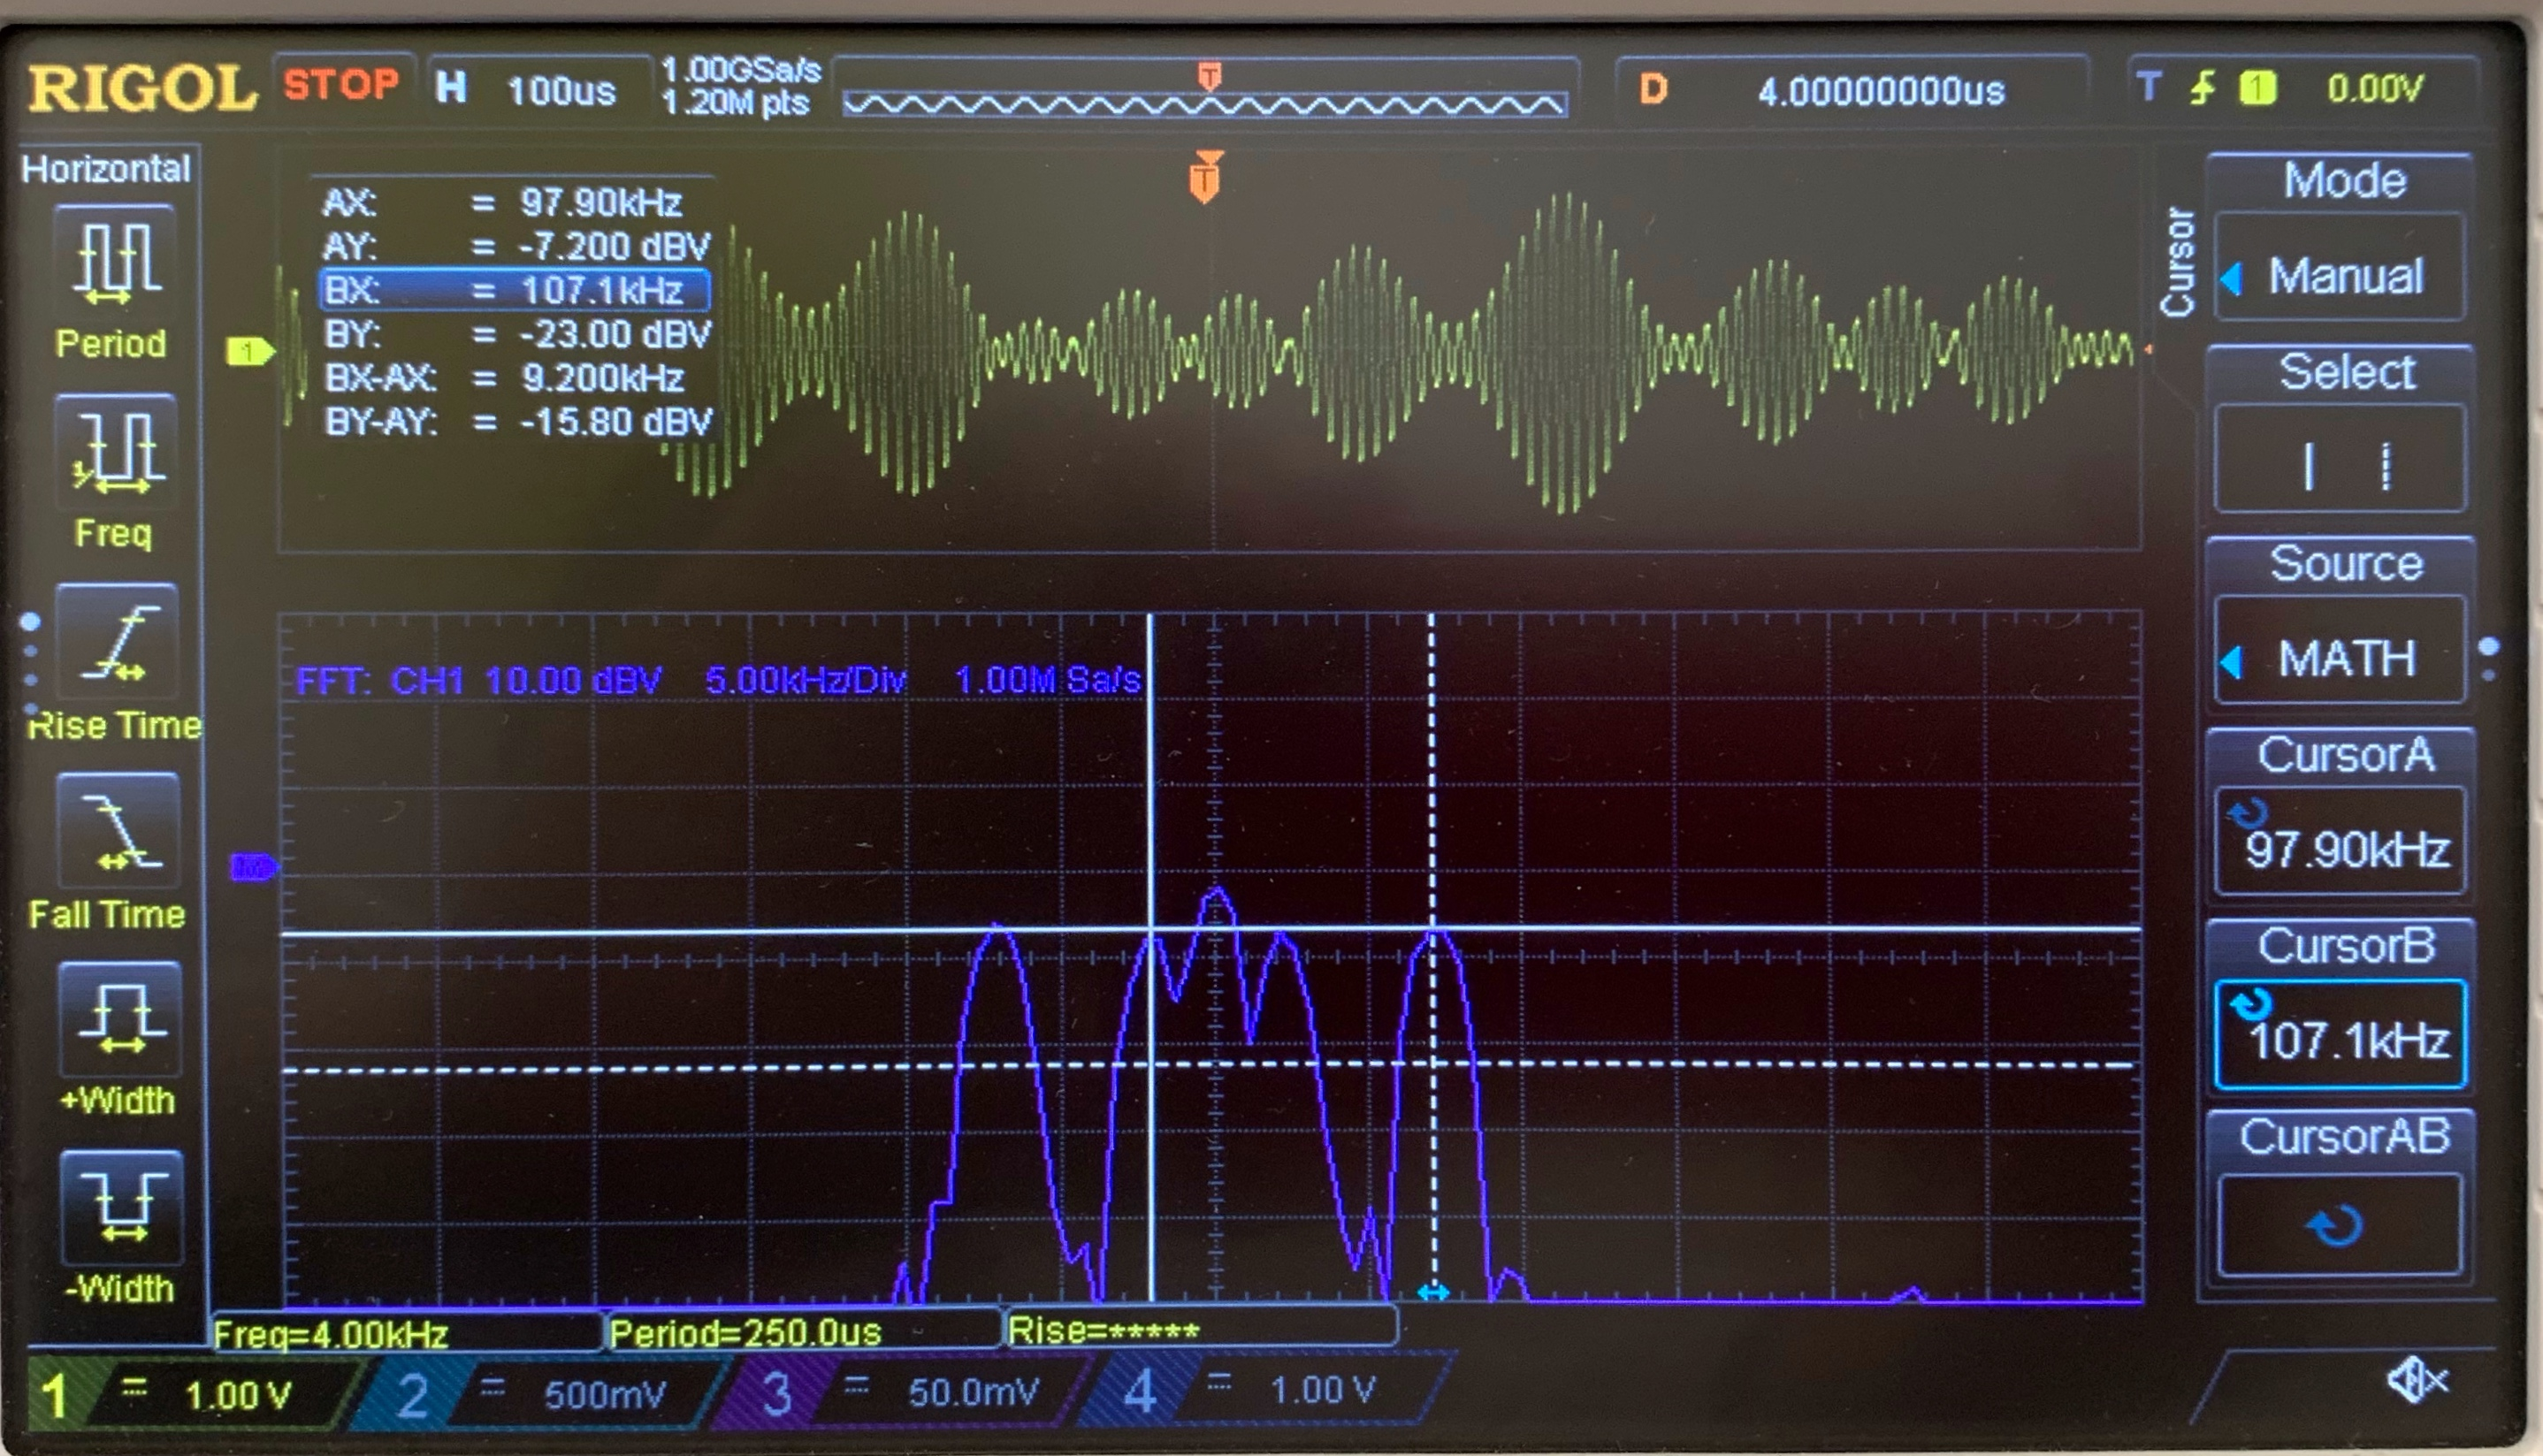
\includegraphics[scale = 0.15]{Q4bLmu.jpg}
    \caption{\label{fig:q4bsmall}AM modulated signal $s_{AM}(t)$ with $\mu$ smaller than maximum value.}
\end{figure}
\begin{figure}[H]
    \centering
    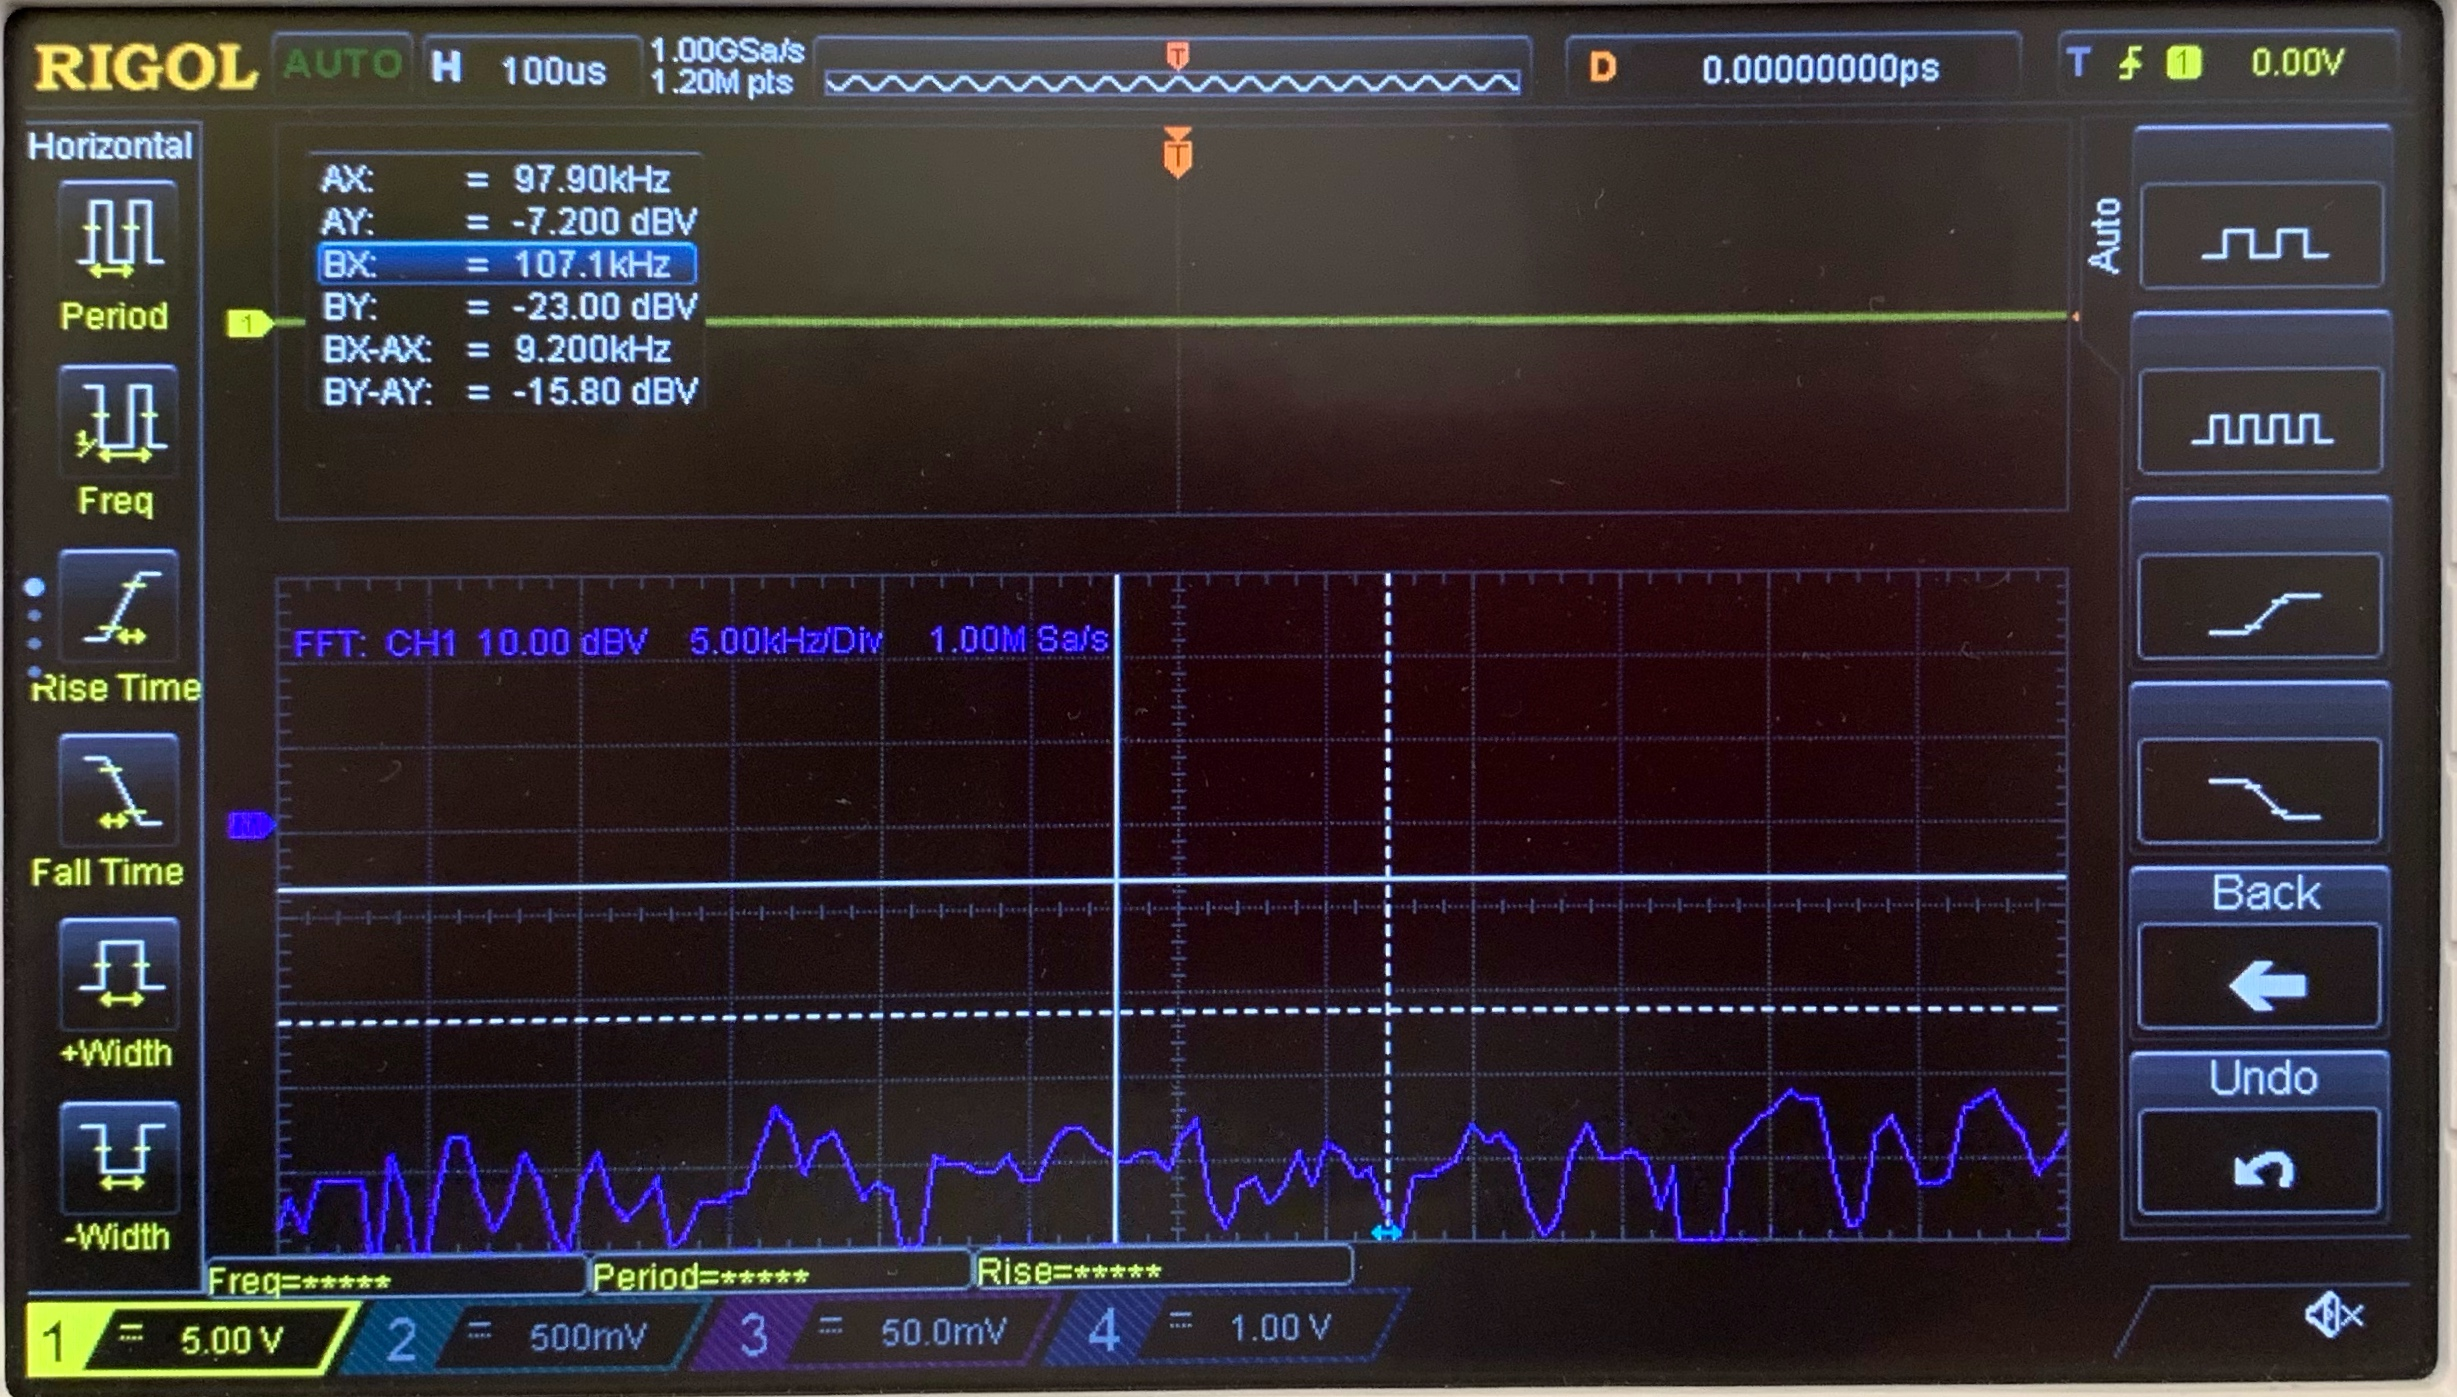
\includegraphics[scale = 0.175]{Q4bSmu.jpg}
    \caption{\label{fig:q4blarge}AM modulated signal $s_{AM} (t)$ with $\mu$ larger than maximum value.}
\end{figure}
As shown in Figure \ref{fig:q4bsmall} and \ref{fig:q4blarge}, $\mu<\frac{32}{33}$ will lead to a desired AM signal while $\mu>\frac{32}{33}$ will lead to distortions. As we turned the modulation index $\mu$ to the far end, there won't be any waveform generated as modulation index $\mu$ is way too high. Theory behind it can be simply interpreted using the envelope of AM signal ($A_c+m(t)$). When $A_c$ is too small, partial envelope will turns to go below x-axis, which leads to distortion. Since $A_c$ is negative proportion to $\mu$, a larger $\mu$ will lead to distortion.  

\item %c 
Please refer to sub-question (b), the graph and analysis of frequency domain graph have been included there.
\end{enumerate}

\section*{Question 5}
\begin{figure}[H]
    \centering
    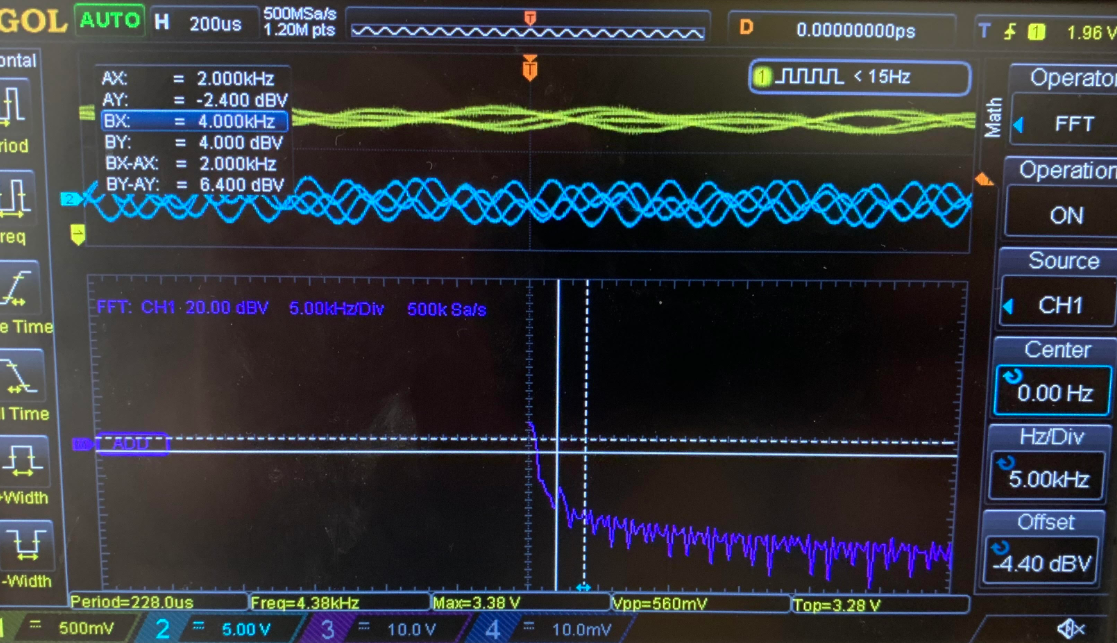
\includegraphics[scale = 0.55]{Q5.PNG}
    \caption{\label{fig:q5}AM Demodulation in time and frequency domain.}
\end{figure}
The AM signal $s_{AM}(t)$ has been demodulated following instructions and the time/frequency domain waveform has been shown in Figure \ref{fig:q5}. It can be seen that the spectrum has contained significant frequency components near baseband which is a property of a message signal. Due to the time constrain, time-domain signal has not been scaled up to see its similarity with the original message signal. But from the aspect of spectrum performance, it seems that the demodulated signal is resembling the original message signal $m(t)$. 

\section*{Question 6}
Due to time limitations we could not experimentally complete this section. However, to our knowledge of the speech module, it will output a "message" signal similar to Figure \ref{fig:q6} from recorded speech. We have demonstrated the DSBSC/AM modulations and respective FFT transforms for a 3.5 second speech signal we recorded in MATLAB. By observing our data, similar outputs should be expected in experimentation. We do note that the TIMS speech module is limited to a 300Hz - 3.4kHz input. With our speech signal as well we can see that AM could be seen as far less efficient due to the non-suppressed carrier being transmitted. 
\begin{figure}[H]
    \centering
    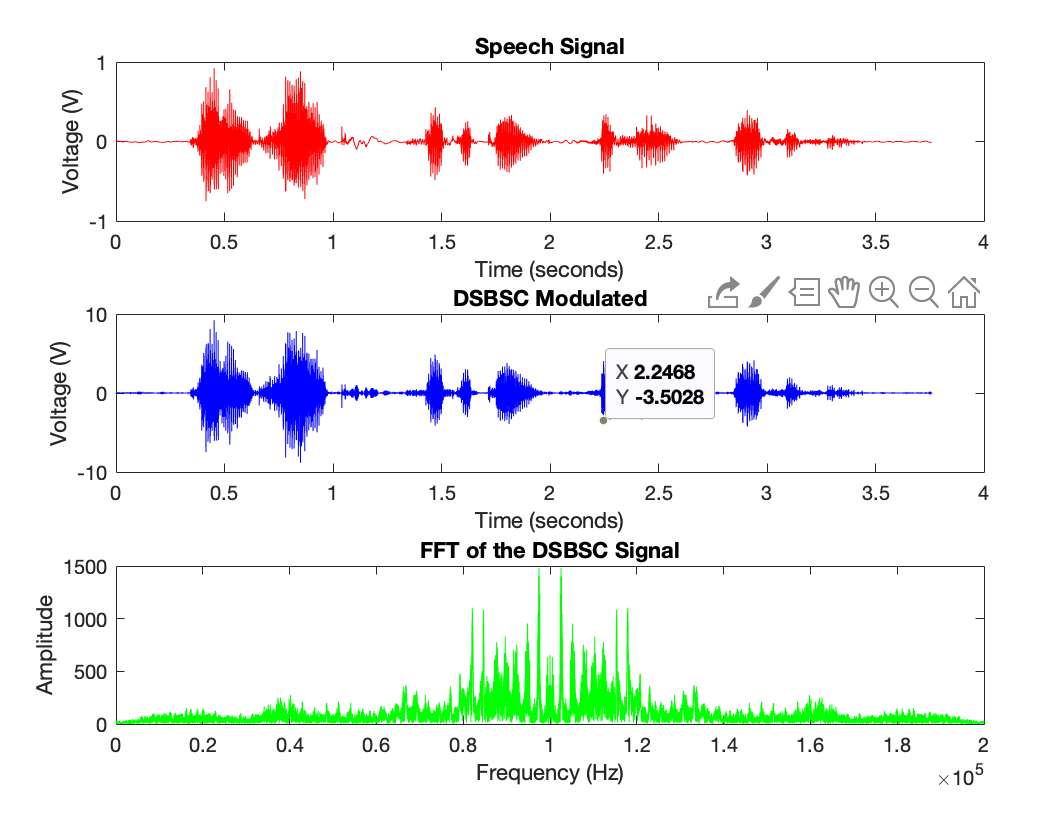
\includegraphics[scale=0.4]{W2Q6DSBSC.png}
    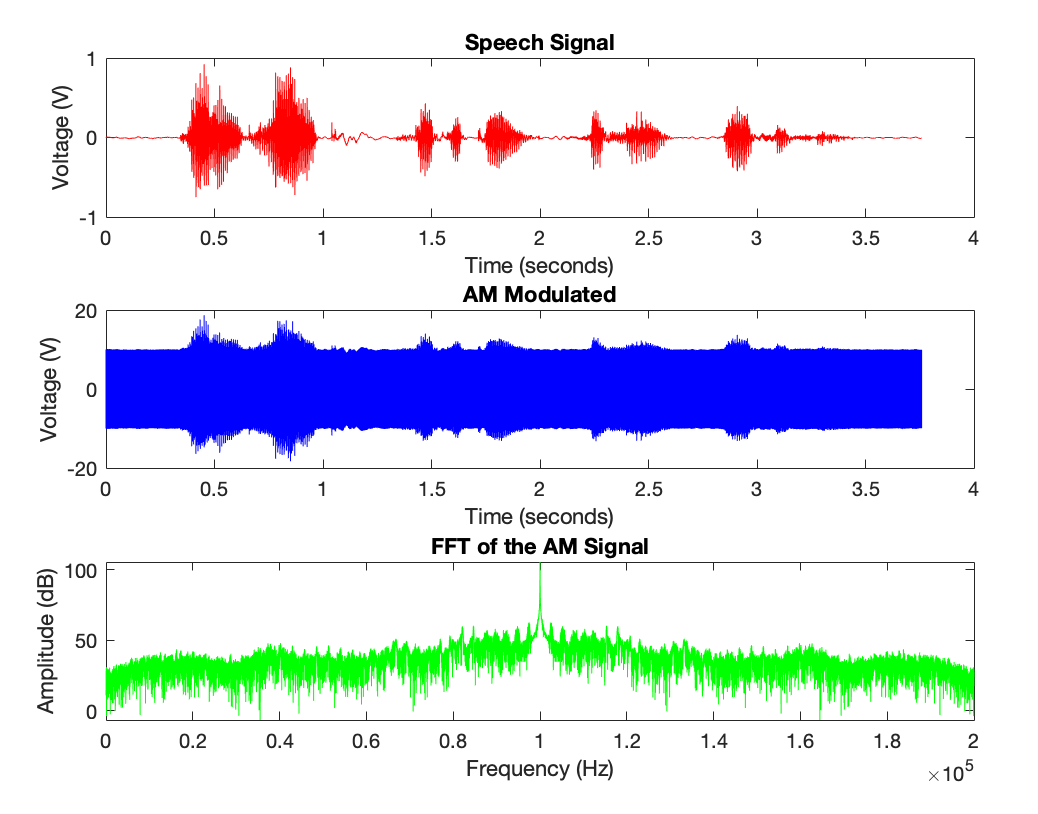
\includegraphics[scale=0.4]{W2Q6AM.png}
    \caption{a) DSBSC modulated signal b) AM modulated signal}
    \label{fig:q6}
\end{figure}

\section*{MATLAB Code for Q6}
\begin{lstlisting}[frame=single]
 % Plotting for Q6 Comm Sys
% Speech signal is derived from recorded sound wave speech.wav
load('speech.mat')
Ac = 10;
fc = 100000;
ts = 1/fs;
n = [1:length(data)];
Carrier = Ac*cos(2*pi*fc*n*ts);

DSBSC = Carrier.*data';
DSBSC_fft = fft(DSBSC);

mu = 31/33; % smaller than technical maximum of 32/33
AM = Carrier + mu*DSBSC;
AM_fft = fft(AM);

%% Plotting the graph
plot_x = n*ts;
plot_fftx = n*(2*fc/length(data));
% DSBSC
figure(1);
set(gcf,'color','w');
subplot(3,1,1)
plot(plot_x,data,'r')
title('Speech Signal');
xlabel('Time (seconds)')
ylabel('Voltage (V)')
subplot(3,1,2)
plot(plot_x,DSBSC,'b')
title('DSBSC Modulated');
xlabel('Time (seconds)')
ylabel('Voltage (V)')
subplot(3,1,3)
plot(plot_fftx,abs(DSBSC_fft),'g');
title('FFT of the DSBSC Signal')
xlabel('Frequency (Hz)')
ylabel('Amplitude')
% AM
figure(2);
set(gcf,'color','w');
subplot(3,1,1)
plot(plot_x,data,'r')
title('Speech Signal');
xlabel('Time (seconds)')
ylabel('Voltage (V)')
subplot(3,1,2)
plot(plot_x,AM,'b')
title('AM Modulated');
xlabel('Time (seconds)')
ylabel('Voltage (V)')
subplot(3,1,3)
plot(plot_fftx,db(abs(AM_fft)),'g');
title('FFT of the AM Signal')
xlabel('Frequency (Hz)')
ylabel('Amplitude (dB)')
\end{lstlisting}

\section*{Check-offs}
Please kindly find check-offs on the following pages.
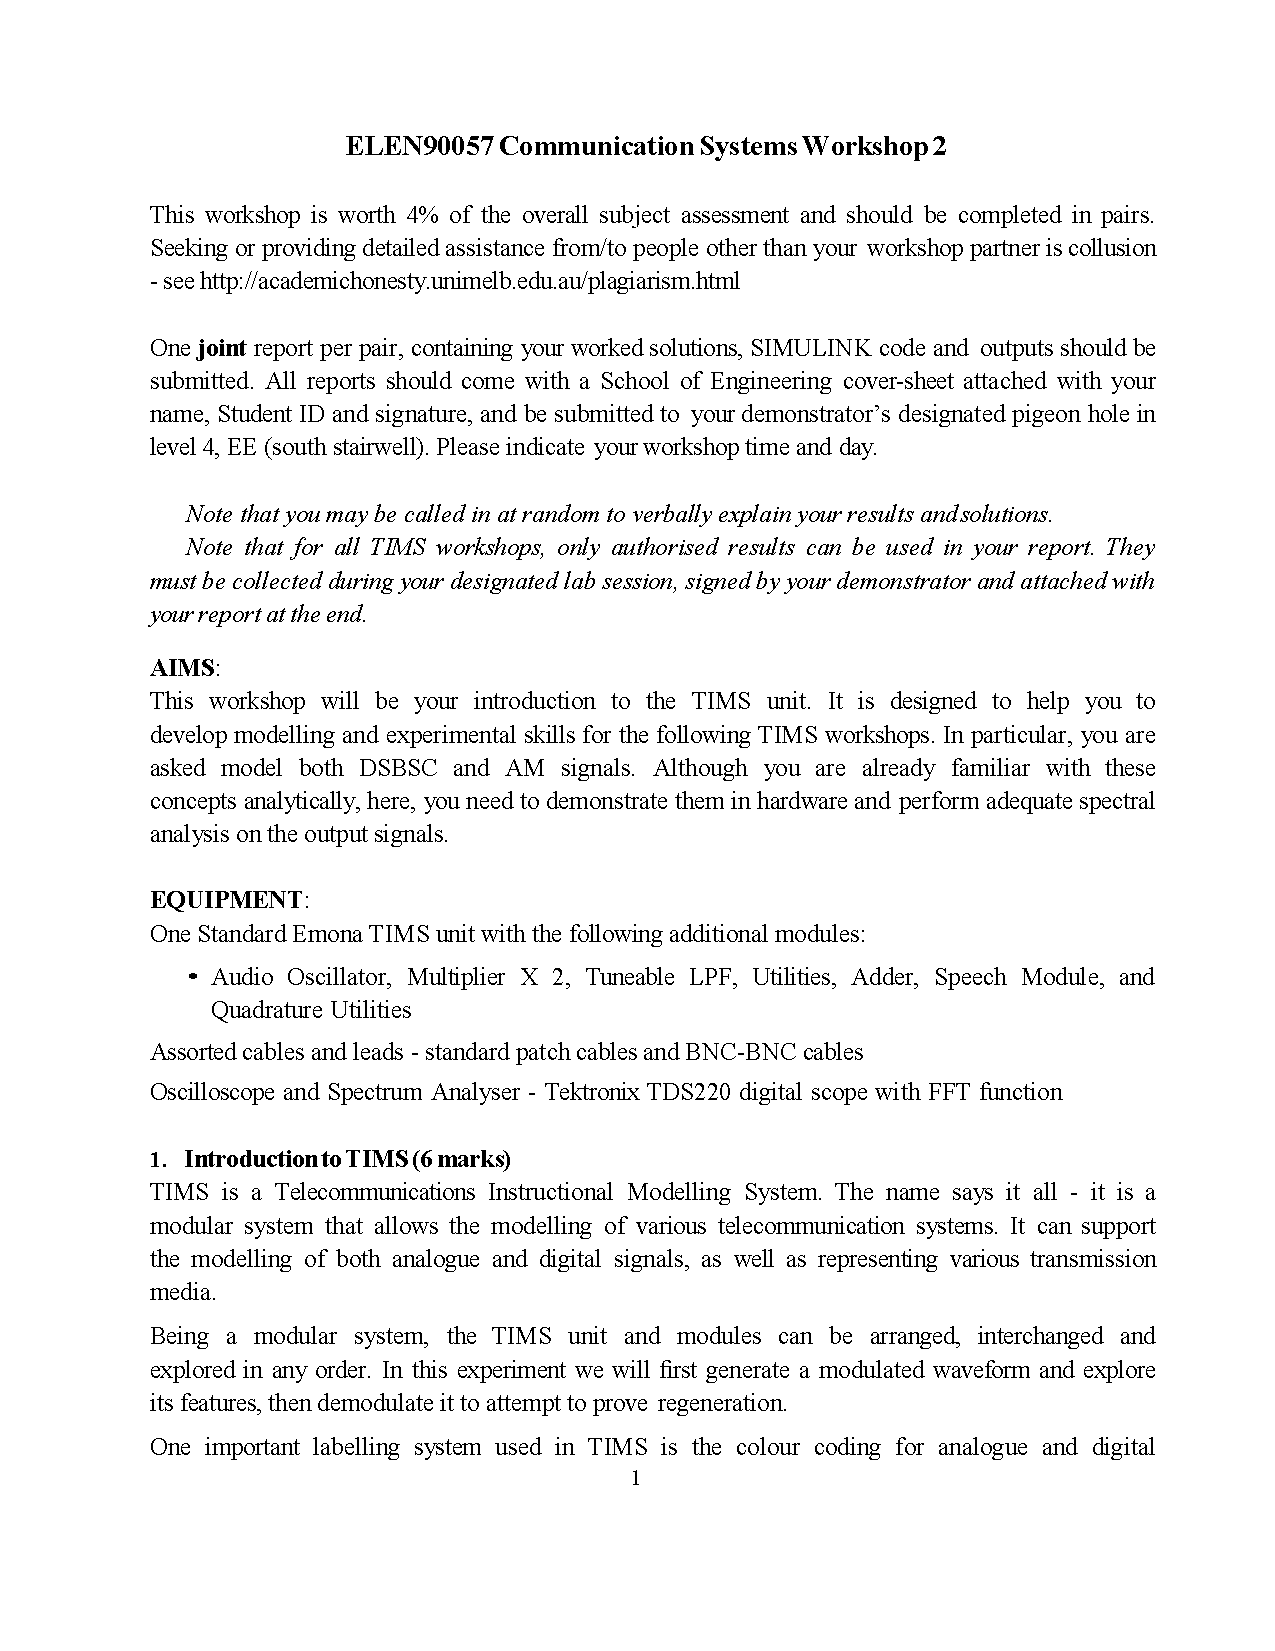
\includepdf[pages={1-},scale=1]{WS2.pdf}
\end{document}
